% Options for packages loaded elsewhere
\PassOptionsToPackage{unicode}{hyperref}
\PassOptionsToPackage{hyphens}{url}
%
\documentclass[
]{article}
\usepackage{amsmath,amssymb}
\usepackage{iftex}
\ifPDFTeX
  \usepackage[T1]{fontenc}
  \usepackage[utf8]{inputenc}
  \usepackage{textcomp} % provide euro and other symbols
\else % if luatex or xetex
  \usepackage{unicode-math} % this also loads fontspec
  \defaultfontfeatures{Scale=MatchLowercase}
  \defaultfontfeatures[\rmfamily]{Ligatures=TeX,Scale=1}
\fi
\usepackage{lmodern}
\ifPDFTeX\else
  % xetex/luatex font selection
\fi
% Use upquote if available, for straight quotes in verbatim environments
\IfFileExists{upquote.sty}{\usepackage{upquote}}{}
\IfFileExists{microtype.sty}{% use microtype if available
  \usepackage[]{microtype}
  \UseMicrotypeSet[protrusion]{basicmath} % disable protrusion for tt fonts
}{}
\makeatletter
\@ifundefined{KOMAClassName}{% if non-KOMA class
  \IfFileExists{parskip.sty}{%
    \usepackage{parskip}
  }{% else
    \setlength{\parindent}{0pt}
    \setlength{\parskip}{6pt plus 2pt minus 1pt}}
}{% if KOMA class
  \KOMAoptions{parskip=half}}
\makeatother
\usepackage{xcolor}
\usepackage[margin=1in]{geometry}
\usepackage{color}
\usepackage{fancyvrb}
\newcommand{\VerbBar}{|}
\newcommand{\VERB}{\Verb[commandchars=\\\{\}]}
\DefineVerbatimEnvironment{Highlighting}{Verbatim}{commandchars=\\\{\}}
% Add ',fontsize=\small' for more characters per line
\usepackage{framed}
\definecolor{shadecolor}{RGB}{248,248,248}
\newenvironment{Shaded}{\begin{snugshade}}{\end{snugshade}}
\newcommand{\AlertTok}[1]{\textcolor[rgb]{0.94,0.16,0.16}{#1}}
\newcommand{\AnnotationTok}[1]{\textcolor[rgb]{0.56,0.35,0.01}{\textbf{\textit{#1}}}}
\newcommand{\AttributeTok}[1]{\textcolor[rgb]{0.13,0.29,0.53}{#1}}
\newcommand{\BaseNTok}[1]{\textcolor[rgb]{0.00,0.00,0.81}{#1}}
\newcommand{\BuiltInTok}[1]{#1}
\newcommand{\CharTok}[1]{\textcolor[rgb]{0.31,0.60,0.02}{#1}}
\newcommand{\CommentTok}[1]{\textcolor[rgb]{0.56,0.35,0.01}{\textit{#1}}}
\newcommand{\CommentVarTok}[1]{\textcolor[rgb]{0.56,0.35,0.01}{\textbf{\textit{#1}}}}
\newcommand{\ConstantTok}[1]{\textcolor[rgb]{0.56,0.35,0.01}{#1}}
\newcommand{\ControlFlowTok}[1]{\textcolor[rgb]{0.13,0.29,0.53}{\textbf{#1}}}
\newcommand{\DataTypeTok}[1]{\textcolor[rgb]{0.13,0.29,0.53}{#1}}
\newcommand{\DecValTok}[1]{\textcolor[rgb]{0.00,0.00,0.81}{#1}}
\newcommand{\DocumentationTok}[1]{\textcolor[rgb]{0.56,0.35,0.01}{\textbf{\textit{#1}}}}
\newcommand{\ErrorTok}[1]{\textcolor[rgb]{0.64,0.00,0.00}{\textbf{#1}}}
\newcommand{\ExtensionTok}[1]{#1}
\newcommand{\FloatTok}[1]{\textcolor[rgb]{0.00,0.00,0.81}{#1}}
\newcommand{\FunctionTok}[1]{\textcolor[rgb]{0.13,0.29,0.53}{\textbf{#1}}}
\newcommand{\ImportTok}[1]{#1}
\newcommand{\InformationTok}[1]{\textcolor[rgb]{0.56,0.35,0.01}{\textbf{\textit{#1}}}}
\newcommand{\KeywordTok}[1]{\textcolor[rgb]{0.13,0.29,0.53}{\textbf{#1}}}
\newcommand{\NormalTok}[1]{#1}
\newcommand{\OperatorTok}[1]{\textcolor[rgb]{0.81,0.36,0.00}{\textbf{#1}}}
\newcommand{\OtherTok}[1]{\textcolor[rgb]{0.56,0.35,0.01}{#1}}
\newcommand{\PreprocessorTok}[1]{\textcolor[rgb]{0.56,0.35,0.01}{\textit{#1}}}
\newcommand{\RegionMarkerTok}[1]{#1}
\newcommand{\SpecialCharTok}[1]{\textcolor[rgb]{0.81,0.36,0.00}{\textbf{#1}}}
\newcommand{\SpecialStringTok}[1]{\textcolor[rgb]{0.31,0.60,0.02}{#1}}
\newcommand{\StringTok}[1]{\textcolor[rgb]{0.31,0.60,0.02}{#1}}
\newcommand{\VariableTok}[1]{\textcolor[rgb]{0.00,0.00,0.00}{#1}}
\newcommand{\VerbatimStringTok}[1]{\textcolor[rgb]{0.31,0.60,0.02}{#1}}
\newcommand{\WarningTok}[1]{\textcolor[rgb]{0.56,0.35,0.01}{\textbf{\textit{#1}}}}
\usepackage{graphicx}
\makeatletter
\def\maxwidth{\ifdim\Gin@nat@width>\linewidth\linewidth\else\Gin@nat@width\fi}
\def\maxheight{\ifdim\Gin@nat@height>\textheight\textheight\else\Gin@nat@height\fi}
\makeatother
% Scale images if necessary, so that they will not overflow the page
% margins by default, and it is still possible to overwrite the defaults
% using explicit options in \includegraphics[width, height, ...]{}
\setkeys{Gin}{width=\maxwidth,height=\maxheight,keepaspectratio}
% Set default figure placement to htbp
\makeatletter
\def\fps@figure{htbp}
\makeatother
\setlength{\emergencystretch}{3em} % prevent overfull lines
\providecommand{\tightlist}{%
  \setlength{\itemsep}{0pt}\setlength{\parskip}{0pt}}
\setcounter{secnumdepth}{-\maxdimen} % remove section numbering
\usepackage{fvextra}
\DefineVerbatimEnvironment{Highlighting}{Verbatim}{
breaklines=true,
commandchars=\\\{\},
fontsize=\normalsize
}
\ifLuaTeX
  \usepackage{selnolig}  % disable illegal ligatures
\fi
\usepackage{bookmark}
\IfFileExists{xurl.sty}{\usepackage{xurl}}{} % add URL line breaks if available
\urlstyle{same}
\hypersetup{
  pdftitle={Saltmarsh Habitat Classification Models},
  pdfauthor={Alyssa Bueno},
  hidelinks,
  pdfcreator={LaTeX via pandoc}}

\title{Saltmarsh Habitat Classification Models}
\author{Alyssa Bueno}
\date{2025-08-02}

\begin{document}
\maketitle

\subsection{Saltmarsh Habitat
Classification}\label{saltmarsh-habitat-classification}

This code outlines 4 different model classification iterations, each
differing by the input layers.

\begin{enumerate}
\def\labelenumi{\arabic{enumi}.}
\tightlist
\item
  NDWI + NDVI + PCA + NAIP + Brightness
\item
  NDWI + NDVI + PCA
\item
  NAIP + NDVI
\item
  PCA
\end{enumerate}

\section{Setup: Ingest the training data and set up the
layers}\label{setup-ingest-the-training-data-and-set-up-the-layers}

\begin{Shaded}
\begin{Highlighting}[]
\CommentTok{\# load raster and training polygons}
\NormalTok{naip }\OtherTok{\textless{}{-}} \FunctionTok{rast}\NormalTok{(}\StringTok{"training\_raster\_round\_6.tif"}\NormalTok{) }\CommentTok{\# this has the raster data    }
\NormalTok{training\_polygons }\OtherTok{\textless{}{-}} \FunctionTok{vect}\NormalTok{(}\StringTok{"training\_polygons\_round\_6.shp"}\NormalTok{) }\CommentTok{\# this has the classes}

\FunctionTok{names}\NormalTok{(naip) }\OtherTok{\textless{}{-}} \FunctionTok{paste0}\NormalTok{(}\StringTok{"naip"}\NormalTok{, }\DecValTok{1}\SpecialCharTok{:}\DecValTok{4}\NormalTok{) }\CommentTok{\# change name of naip bands layer}

\CommentTok{\# calculate NDVI}
\NormalTok{ndvi }\OtherTok{\textless{}{-}}\NormalTok{ (naip[[}\DecValTok{4}\NormalTok{]] }\SpecialCharTok{{-}}\NormalTok{ naip[[}\DecValTok{1}\NormalTok{]]) }\SpecialCharTok{/}\NormalTok{ (naip[[}\DecValTok{4}\NormalTok{]] }\SpecialCharTok{+}\NormalTok{ naip[[}\DecValTok{1}\NormalTok{]])}
\FunctionTok{names}\NormalTok{(ndvi) }\OtherTok{\textless{}{-}} \StringTok{"ndvi"}

\CommentTok{\# calculate brightness}
\NormalTok{brightness }\OtherTok{\textless{}{-}}\NormalTok{ (naip[[}\DecValTok{1}\NormalTok{]] }\SpecialCharTok{+}\NormalTok{ naip[[}\DecValTok{2}\NormalTok{]] }\SpecialCharTok{+}\NormalTok{ naip[[}\DecValTok{3}\NormalTok{]] }\SpecialCharTok{+}\NormalTok{ naip[[}\DecValTok{4}\NormalTok{]]) }\SpecialCharTok{/} \DecValTok{4}
\FunctionTok{names}\NormalTok{(brightness) }\OtherTok{\textless{}{-}} \StringTok{"brightness"}

\CommentTok{\# calculate ndwi}
\NormalTok{ndwi }\OtherTok{\textless{}{-}}\NormalTok{ (naip[[}\DecValTok{4}\NormalTok{]] }\SpecialCharTok{{-}}\NormalTok{ naip[[}\DecValTok{2}\NormalTok{]]) }\SpecialCharTok{/}\NormalTok{ (naip[[}\DecValTok{4}\NormalTok{]] }\SpecialCharTok{+}\NormalTok{ naip[[}\DecValTok{2}\NormalTok{]])}
\FunctionTok{names}\NormalTok{(ndwi) }\OtherTok{\textless{}{-}} \StringTok{"ndwi"}

\CommentTok{\# now create the PCA }

\NormalTok{all\_for\_pca }\OtherTok{\textless{}{-}} \FunctionTok{c}\NormalTok{(naip, ndvi)  }\CommentTok{\# add ndvi to the raster}
\NormalTok{vals }\OtherTok{\textless{}{-}} \FunctionTok{values}\NormalTok{(all\_for\_pca)}
\NormalTok{vals }\OtherTok{\textless{}{-}}\NormalTok{ vals[}\FunctionTok{complete.cases}\NormalTok{(vals), ]}
\NormalTok{pca\_pixels }\OtherTok{\textless{}{-}} \FunctionTok{prcomp}\NormalTok{(vals, }\AttributeTok{center =} \ConstantTok{TRUE}\NormalTok{, }\AttributeTok{scale. =} \ConstantTok{TRUE}\NormalTok{)}
\NormalTok{pca }\OtherTok{\textless{}{-}} \FunctionTok{predict}\NormalTok{(all\_for\_pca, pca\_pixels, }\AttributeTok{index =} \DecValTok{1}\SpecialCharTok{:}\DecValTok{5}\NormalTok{)  }\CommentTok{\# for 5 PCs}
\end{Highlighting}
\end{Shaded}

\begin{verbatim}
## |---------|---------|---------|---------|=========================================                                          
\end{verbatim}

\begin{Shaded}
\begin{Highlighting}[]
\FunctionTok{names}\NormalTok{(pca) }\OtherTok{\textless{}{-}} \FunctionTok{paste0}\NormalTok{(}\StringTok{"PCA"}\NormalTok{, }\DecValTok{1}\SpecialCharTok{:}\DecValTok{5}\NormalTok{)}
\end{Highlighting}
\end{Shaded}

\section{1. First Iteration: NDWI + NDVI + PCA + NAIP +
Brightness}\label{first-iteration-ndwi-ndvi-pca-naip-brightness}

\begin{Shaded}
\begin{Highlighting}[]
\CommentTok{\# stack em up}
\NormalTok{r\_stack }\OtherTok{\textless{}{-}} \FunctionTok{c}\NormalTok{(ndwi, ndvi, pca, naip, brightness)}

\CommentTok{\# extract raster values for training polygons}
\NormalTok{extracted }\OtherTok{\textless{}{-}}\NormalTok{ terra}\SpecialCharTok{::}\FunctionTok{extract}\NormalTok{(r\_stack, training\_polygons, }\AttributeTok{df =} \ConstantTok{TRUE}\NormalTok{)}

\CommentTok{\# turn class into a factor}
\NormalTok{training\_polygons}\SpecialCharTok{$}\NormalTok{class }\OtherTok{\textless{}{-}} \FunctionTok{as.factor}\NormalTok{(training\_polygons}\SpecialCharTok{$}\NormalTok{class)}

\CommentTok{\# Convert training\_polygons to dataframe to get the class labels}
\NormalTok{poly\_df }\OtherTok{\textless{}{-}} \FunctionTok{as.data.frame}\NormalTok{(training\_polygons)}
\NormalTok{poly\_df}\SpecialCharTok{$}\NormalTok{ID }\OtherTok{\textless{}{-}} \DecValTok{1}\SpecialCharTok{:}\FunctionTok{nrow}\NormalTok{(poly\_df)  }\CommentTok{\# Add ID column to match extract output}

\CommentTok{\# Join the class labels}
\NormalTok{extracted }\OtherTok{\textless{}{-}}\NormalTok{ extracted }\SpecialCharTok{\%\textgreater{}\%}
  \FunctionTok{left\_join}\NormalTok{(poly\_df[, }\FunctionTok{c}\NormalTok{(}\StringTok{"ID"}\NormalTok{, }\StringTok{"class"}\NormalTok{)], }\AttributeTok{by =} \StringTok{"ID"}\NormalTok{)}

\CommentTok{\# clean data by removing rows with na values and remove ID column}
\NormalTok{extracted\_clean }\OtherTok{\textless{}{-}} \FunctionTok{na.omit}\NormalTok{(extracted[, }\SpecialCharTok{{-}}\DecValTok{1}\NormalTok{])  }\CommentTok{\# remove ID and NAs}

\CommentTok{\# sample 2000 per class}
\NormalTok{training\_data }\OtherTok{\textless{}{-}}\NormalTok{ extracted\_clean }\SpecialCharTok{\%\textgreater{}\%}
  \FunctionTok{group\_by}\NormalTok{(class) }\SpecialCharTok{\%\textgreater{}\%}
  \FunctionTok{sample\_n}\NormalTok{(}\FunctionTok{min}\NormalTok{(}\DecValTok{2000}\NormalTok{, }\FunctionTok{n}\NormalTok{())) }\SpecialCharTok{\%\textgreater{}\%}  \CommentTok{\# Use min() to handle small classes}
  \FunctionTok{ungroup}\NormalTok{()}

\CommentTok{\# turn class column into factor}
\NormalTok{training\_data}\SpecialCharTok{$}\NormalTok{class }\OtherTok{\textless{}{-}} \FunctionTok{factor}\NormalTok{(training\_data}\SpecialCharTok{$}\NormalTok{class)}

\CommentTok{\# check the sampling balance in the classes}
\FunctionTok{print}\NormalTok{(}\FunctionTok{table}\NormalTok{(training\_data}\SpecialCharTok{$}\NormalTok{class))}
\end{Highlighting}
\end{Shaded}

\begin{verbatim}
## 
##   hm   lm   md   ow   ph   rd   up 
## 2000 2000 2000 2000 2000 2000 2000
\end{verbatim}

\begin{Shaded}
\begin{Highlighting}[]
\CommentTok{\# split training and test data}
\FunctionTok{set.seed}\NormalTok{(}\DecValTok{342}\NormalTok{)}
\NormalTok{idx }\OtherTok{\textless{}{-}} \FunctionTok{sample}\NormalTok{(}\FunctionTok{seq\_len}\NormalTok{(}\FunctionTok{nrow}\NormalTok{(training\_data)), }\AttributeTok{size =} \FloatTok{0.8} \SpecialCharTok{*} \FunctionTok{nrow}\NormalTok{(training\_data))}
\NormalTok{train\_set }\OtherTok{\textless{}{-}}\NormalTok{ training\_data[idx, ]}
\NormalTok{test\_set  }\OtherTok{\textless{}{-}}\NormalTok{ training\_data[}\SpecialCharTok{{-}}\NormalTok{idx, ]}

\CommentTok{\# train random forest model}
\NormalTok{rf\_model }\OtherTok{\textless{}{-}} \FunctionTok{randomForest}\NormalTok{(class }\SpecialCharTok{\textasciitilde{}}\NormalTok{ ., }
                         \AttributeTok{data =}\NormalTok{ train\_set, }
                         \AttributeTok{ntree =} \DecValTok{500}\NormalTok{)}

\CommentTok{\# validation metrics}
\NormalTok{preds }\OtherTok{\textless{}{-}} \FunctionTok{predict}\NormalTok{(rf\_model, }\AttributeTok{newdata =}\NormalTok{ test\_set)}
\NormalTok{accuracy }\OtherTok{\textless{}{-}} \FunctionTok{mean}\NormalTok{(preds }\SpecialCharTok{==}\NormalTok{ test\_set}\SpecialCharTok{$}\NormalTok{class)}
\FunctionTok{cat}\NormalTok{(}\StringTok{"Accuracy:"}\NormalTok{, }\FunctionTok{round}\NormalTok{(accuracy, }\DecValTok{4}\NormalTok{), }\StringTok{"}\SpecialCharTok{\textbackslash{}n}\StringTok{"}\NormalTok{)}
\end{Highlighting}
\end{Shaded}

\begin{verbatim}
## Accuracy: 0.9721
\end{verbatim}

\begin{Shaded}
\begin{Highlighting}[]
\FunctionTok{print}\NormalTok{(rf\_model)}
\end{Highlighting}
\end{Shaded}

\begin{verbatim}
## 
## Call:
##  randomForest(formula = class ~ ., data = train_set, ntree = 500) 
##                Type of random forest: classification
##                      Number of trees: 500
## No. of variables tried at each split: 3
## 
##         OOB estimate of  error rate: 2.12%
## Confusion matrix:
##      hm   lm   md   ow   ph   rd   up class.error
## hm 1596    8    0    0    1    2    0 0.006845053
## lm   13 1554    5    0   24    0    1 0.026925485
## md    0    2 1563    0    0   36    0 0.023735166
## ow    0    0    0 1589    0    0    0 0.000000000
## ph    0   34    0    0 1564    2   12 0.029776675
## rd    2    0   47    0   12 1543    1 0.038629283
## up    3   16    0    0   16    0 1554 0.022026432
\end{verbatim}

\begin{Shaded}
\begin{Highlighting}[]
\CommentTok{\# confusion matrix}
\FunctionTok{confusionMatrix}\NormalTok{(preds, test\_set}\SpecialCharTok{$}\NormalTok{class)}
\end{Highlighting}
\end{Shaded}

\begin{verbatim}
## Confusion Matrix and Statistics
## 
##           Reference
## Prediction  hm  lm  md  ow  ph  rd  up
##         hm 388   4   0   0   0   1   0
##         lm   4 390   2   0  10   1   6
##         md   0   0 383   0   0  15   0
##         ow   0   0   0 411   0   0   0
##         ph   0   9   0   0 377   2   8
##         rd   1   0  14   0   0 376   0
##         up   0   0   0   0   1   0 397
## 
## Overall Statistics
##                                           
##                Accuracy : 0.9721          
##                  95% CI : (0.9654, 0.9779)
##     No Information Rate : 0.1468          
##     P-Value [Acc > NIR] : < 2.2e-16       
##                                           
##                   Kappa : 0.9675          
##                                           
##  Mcnemar's Test P-Value : NA              
## 
## Statistics by Class:
## 
##                      Class: hm Class: lm Class: md Class: ow Class: ph
## Sensitivity             0.9873    0.9677    0.9599    1.0000    0.9716
## Specificity             0.9979    0.9904    0.9938    1.0000    0.9921
## Pos Pred Value          0.9873    0.9443    0.9623    1.0000    0.9520
## Neg Pred Value          0.9979    0.9946    0.9933    1.0000    0.9954
## Prevalence              0.1404    0.1439    0.1425    0.1468    0.1386
## Detection Rate          0.1386    0.1393    0.1368    0.1468    0.1346
## Detection Prevalence    0.1404    0.1475    0.1421    0.1468    0.1414
## Balanced Accuracy       0.9926    0.9791    0.9768    1.0000    0.9819
##                      Class: rd Class: up
## Sensitivity             0.9519    0.9659
## Specificity             0.9938    0.9996
## Pos Pred Value          0.9616    0.9975
## Neg Pred Value          0.9921    0.9942
## Prevalence              0.1411    0.1468
## Detection Rate          0.1343    0.1418
## Detection Prevalence    0.1396    0.1421
## Balanced Accuracy       0.9728    0.9828
\end{verbatim}

\section{classifying the plots}\label{classifying-the-plots}

\begin{Shaded}
\begin{Highlighting}[]
\CommentTok{\# load the new, unlabeled raster}
\NormalTok{prediction\_raster }\OtherTok{\textless{}{-}} \FunctionTok{rast}\NormalTok{(}\StringTok{"\textasciitilde{}/Desktop/marshbirdsoutput/round\_6/prediction\_raster\_round\_6.tif"}\NormalTok{)}

\CommentTok{\# calculate NDVI for prediction raster}
\NormalTok{ndvi\_pred }\OtherTok{\textless{}{-}}\NormalTok{ (prediction\_raster[[}\DecValTok{4}\NormalTok{]] }\SpecialCharTok{{-}}\NormalTok{ prediction\_raster[[}\DecValTok{1}\NormalTok{]]) }\SpecialCharTok{/} 
\NormalTok{  (prediction\_raster[[}\DecValTok{4}\NormalTok{]] }\SpecialCharTok{+}\NormalTok{ prediction\_raster[[}\DecValTok{1}\NormalTok{]])}
\FunctionTok{names}\NormalTok{(ndvi\_pred) }\OtherTok{\textless{}{-}} \StringTok{"ndvi"}

\CommentTok{\# calculation NDWI}
\NormalTok{ndwi\_pred }\OtherTok{\textless{}{-}}\NormalTok{ (prediction\_raster[[}\DecValTok{4}\NormalTok{]] }\SpecialCharTok{{-}}\NormalTok{ prediction\_raster[[}\DecValTok{2}\NormalTok{]]) }\SpecialCharTok{/} 
\NormalTok{  (prediction\_raster[[}\DecValTok{4}\NormalTok{]] }\SpecialCharTok{+}\NormalTok{ prediction\_raster[[}\DecValTok{2}\NormalTok{]])}
\FunctionTok{names}\NormalTok{(ndwi\_pred) }\OtherTok{\textless{}{-}} \StringTok{"ndwi"}

\CommentTok{\# Calculate brightness}
\NormalTok{brightness\_pred }\OtherTok{\textless{}{-}}\NormalTok{ (prediction\_raster[[}\DecValTok{1}\NormalTok{]] }\SpecialCharTok{+}\NormalTok{ prediction\_raster[[}\DecValTok{2}\NormalTok{]] }\SpecialCharTok{+} 
\NormalTok{                      prediction\_raster[[}\DecValTok{3}\NormalTok{]] }\SpecialCharTok{+}\NormalTok{ prediction\_raster[[}\DecValTok{4}\NormalTok{]]) }\SpecialCharTok{/} \DecValTok{4}
\FunctionTok{names}\NormalTok{(brightness\_pred) }\OtherTok{\textless{}{-}} \StringTok{"brightness"}

\CommentTok{\# Apply the pca}
\NormalTok{all\_for\_pca\_pred }\OtherTok{\textless{}{-}} \FunctionTok{c}\NormalTok{(prediction\_raster, ndvi\_pred)}
\FunctionTok{names}\NormalTok{(all\_for\_pca\_pred) }\OtherTok{\textless{}{-}} \FunctionTok{names}\NormalTok{(all\_for\_pca)  }\CommentTok{\# ensure exact match}
\NormalTok{pca\_pred }\OtherTok{\textless{}{-}} \FunctionTok{predict}\NormalTok{(all\_for\_pca\_pred, pca\_pixels, }\AttributeTok{index =} \DecValTok{1}\SpecialCharTok{:}\DecValTok{5}\NormalTok{)}
\end{Highlighting}
\end{Shaded}

\begin{verbatim}
## |---------|---------|---------|---------|=========================================                                          
\end{verbatim}

\begin{Shaded}
\begin{Highlighting}[]
\FunctionTok{names}\NormalTok{(pca\_pred) }\OtherTok{\textless{}{-}} \FunctionTok{paste0}\NormalTok{(}\StringTok{"PCA"}\NormalTok{, }\DecValTok{1}\SpecialCharTok{:}\DecValTok{5}\NormalTok{)}

\CommentTok{\# stack it}
\NormalTok{prediction\_stack }\OtherTok{\textless{}{-}} \FunctionTok{c}\NormalTok{(prediction\_raster, ndvi\_pred, ndwi\_pred, brightness\_pred, pca\_pred)}

\CommentTok{\# rename to match training names}
\FunctionTok{names}\NormalTok{(prediction\_stack) }\OtherTok{\textless{}{-}} \FunctionTok{names}\NormalTok{(r\_stack)}

\CommentTok{\# apply the model to predict classes}
\NormalTok{classified }\OtherTok{\textless{}{-}} \FunctionTok{predict}\NormalTok{(prediction\_stack, rf\_model, }\AttributeTok{na.rm =} \ConstantTok{TRUE}\NormalTok{)}

\CommentTok{\# Define custom colors}
\NormalTok{colors }\OtherTok{\textless{}{-}} \FunctionTok{c}\NormalTok{(}
  \StringTok{"\#a6d96a"}\NormalTok{,  }\CommentTok{\# hm  }
  \StringTok{"\#1a9641"}\NormalTok{,  }\CommentTok{\# lm  }
  \StringTok{"\#8c510a"}\NormalTok{,  }\CommentTok{\# md  }
  \StringTok{"\#3288bd"}\NormalTok{,  }\CommentTok{\# ow  }
  \StringTok{"\#fdae61"}\NormalTok{,  }\CommentTok{\# ph  }
  \StringTok{"\#969696"}\NormalTok{,  }\CommentTok{\# rd  }
  \StringTok{"\#762a83"}   \CommentTok{\# up  }
\NormalTok{)}



\CommentTok{\# Plot with colors}
\FunctionTok{plot}\NormalTok{(classified, }\AttributeTok{col =}\NormalTok{ colors)}
\end{Highlighting}
\end{Shaded}

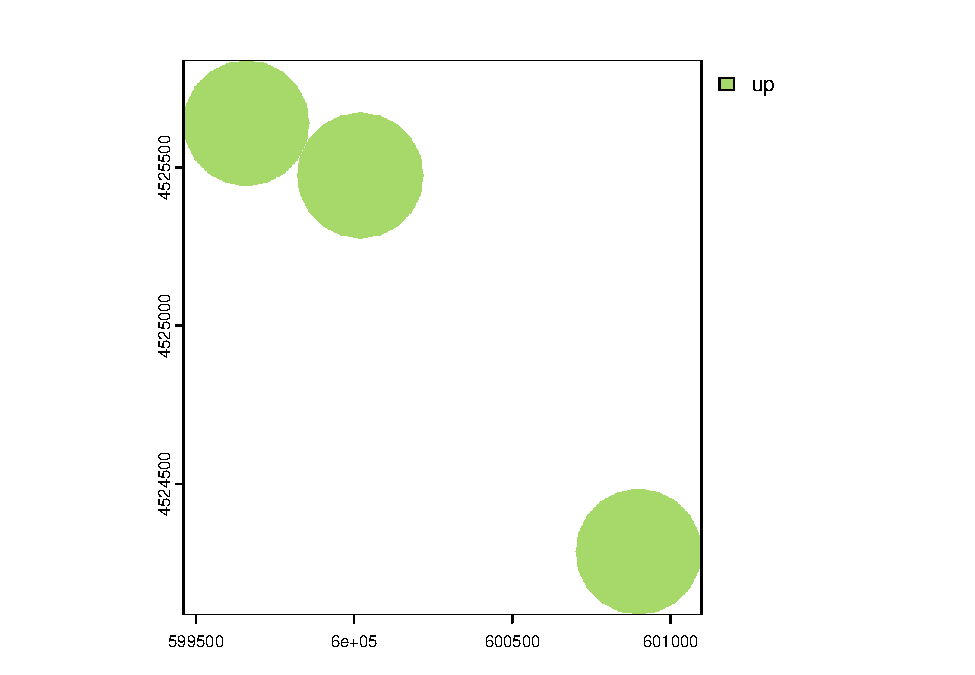
\includegraphics{veg_model_new_class_files/figure-latex/unnamed-chunk-4-1.pdf}

\begin{Shaded}
\begin{Highlighting}[]
\CommentTok{\# save the output tif}
\CommentTok{\# writeRaster(classified, "\textasciitilde{}/Desktop/marshbirdsoutput/round\_6/classified\_output.tif", overwrite = TRUE)}

\NormalTok{rf\_model}\SpecialCharTok{$}\NormalTok{importance}
\end{Highlighting}
\end{Shaded}

\begin{verbatim}
##            MeanDecreaseGini
## ndwi              1342.0737
## ndvi              1257.4674
## PCA1               802.3560
## PCA2               750.9137
## PCA3               540.1606
## PCA4               296.1795
## PCA5               387.6126
## naip1              777.2933
## naip2              482.3840
## naip3              904.0095
## naip4             1230.8604
## brightness         826.3936
\end{verbatim}

\section{feature class importance and
visualizations}\label{feature-class-importance-and-visualizations}

\begin{Shaded}
\begin{Highlighting}[]
\FunctionTok{ggplot}\NormalTok{(training\_data, }\FunctionTok{aes}\NormalTok{(}\AttributeTok{x =}\NormalTok{ ndwi, }\AttributeTok{y =}\NormalTok{ ndvi, }\AttributeTok{color =}\NormalTok{ class)) }\SpecialCharTok{+}
  \FunctionTok{geom\_point}\NormalTok{(}\AttributeTok{alpha =} \FloatTok{0.3}\NormalTok{) }\SpecialCharTok{+}
  \FunctionTok{theme\_minimal}\NormalTok{()}
\end{Highlighting}
\end{Shaded}

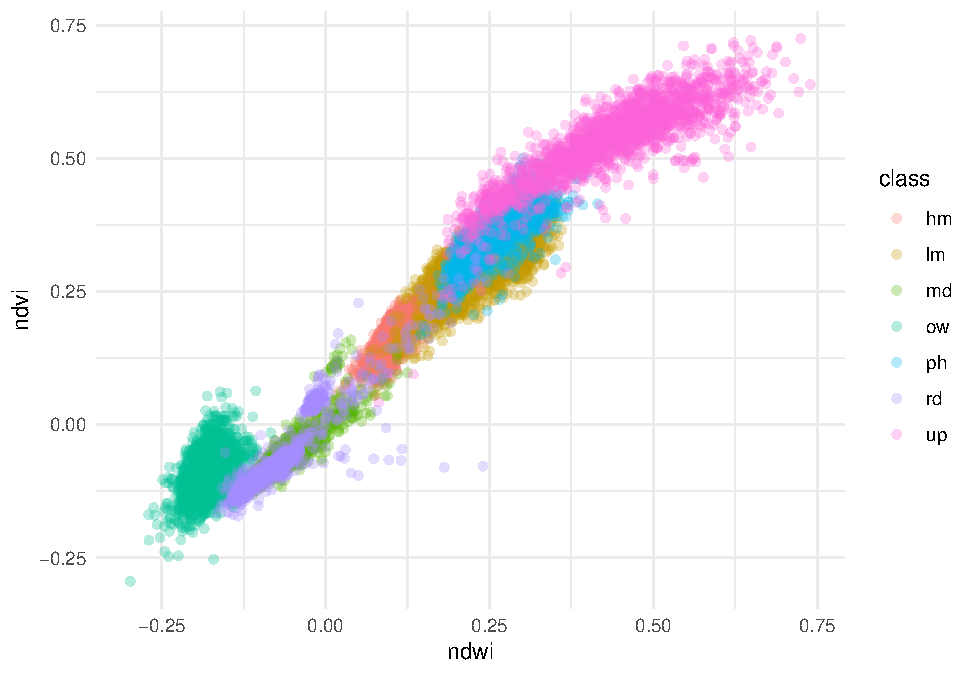
\includegraphics{veg_model_new_class_files/figure-latex/unnamed-chunk-5-1.pdf}

\begin{Shaded}
\begin{Highlighting}[]
\FunctionTok{ggplot}\NormalTok{(training\_data, }\FunctionTok{aes}\NormalTok{(}\AttributeTok{x =}\NormalTok{ ndwi, }\AttributeTok{fill =}\NormalTok{ class)) }\SpecialCharTok{+}
  \FunctionTok{geom\_density}\NormalTok{(}\AttributeTok{alpha =} \FloatTok{0.4}\NormalTok{, }\AttributeTok{color =} \ConstantTok{NA}\NormalTok{) }\SpecialCharTok{+}
  \FunctionTok{theme\_minimal}\NormalTok{()}
\end{Highlighting}
\end{Shaded}

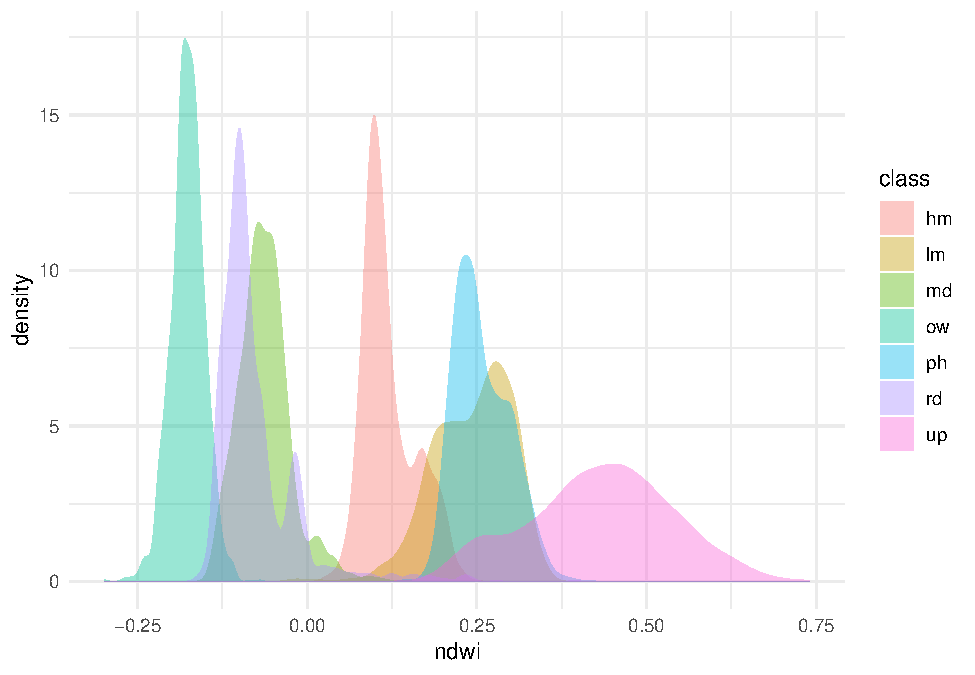
\includegraphics{veg_model_new_class_files/figure-latex/unnamed-chunk-5-2.pdf}

\begin{Shaded}
\begin{Highlighting}[]
\NormalTok{imp }\OtherTok{\textless{}{-}} \FunctionTok{as.data.frame}\NormalTok{(rf\_model}\SpecialCharTok{$}\NormalTok{importance)}
\NormalTok{imp}\SpecialCharTok{$}\NormalTok{feature }\OtherTok{\textless{}{-}} \FunctionTok{rownames}\NormalTok{(imp)}

\FunctionTok{ggplot}\NormalTok{(imp, }\FunctionTok{aes}\NormalTok{(}\AttributeTok{x =} \FunctionTok{reorder}\NormalTok{(feature, MeanDecreaseGini), }\AttributeTok{y =}\NormalTok{ MeanDecreaseGini)) }\SpecialCharTok{+}
  \FunctionTok{geom\_col}\NormalTok{(}\AttributeTok{fill =} \StringTok{"steelblue"}\NormalTok{) }\SpecialCharTok{+}
  \FunctionTok{coord\_flip}\NormalTok{() }\SpecialCharTok{+}
  \FunctionTok{labs}\NormalTok{(}\AttributeTok{title =} \StringTok{"Random Forest Variable Importance"}\NormalTok{,}
       \AttributeTok{x =} \StringTok{"Feature"}\NormalTok{, }\AttributeTok{y =} \StringTok{"Mean Decrease Gini"}\NormalTok{) }\SpecialCharTok{+}
  \FunctionTok{theme\_minimal}\NormalTok{()}
\end{Highlighting}
\end{Shaded}

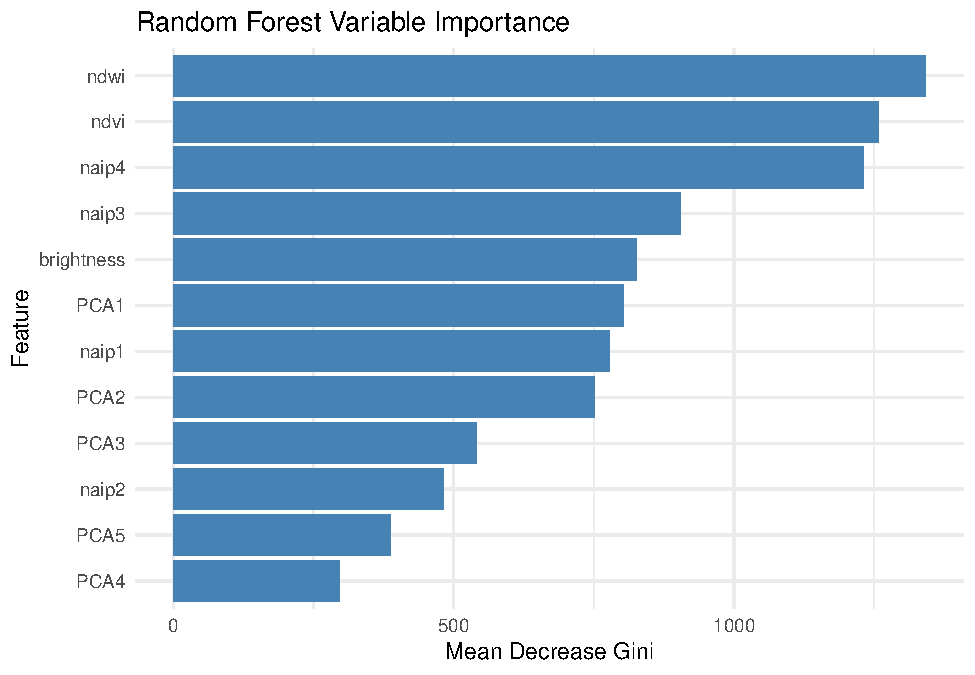
\includegraphics{veg_model_new_class_files/figure-latex/unnamed-chunk-5-3.pdf}

\section{2. Second Iteration: NAIP + NDVI +
NDWI}\label{second-iteration-naip-ndvi-ndwi}

\begin{Shaded}
\begin{Highlighting}[]
\CommentTok{\# stack em up}
\NormalTok{r\_stack }\OtherTok{\textless{}{-}} \FunctionTok{c}\NormalTok{(naip, ndvi, ndwi)}

\CommentTok{\# extract raster values for training polygons}
\NormalTok{extracted }\OtherTok{\textless{}{-}}\NormalTok{ terra}\SpecialCharTok{::}\FunctionTok{extract}\NormalTok{(r\_stack, training\_polygons, }\AttributeTok{df =} \ConstantTok{TRUE}\NormalTok{)}

\CommentTok{\# turn class into a factor}
\NormalTok{training\_polygons}\SpecialCharTok{$}\NormalTok{class }\OtherTok{\textless{}{-}} \FunctionTok{as.factor}\NormalTok{(training\_polygons}\SpecialCharTok{$}\NormalTok{class)}

\CommentTok{\# Convert training\_polygons to dataframe to get the class labels}
\NormalTok{poly\_df }\OtherTok{\textless{}{-}} \FunctionTok{as.data.frame}\NormalTok{(training\_polygons)}
\NormalTok{poly\_df}\SpecialCharTok{$}\NormalTok{ID }\OtherTok{\textless{}{-}} \DecValTok{1}\SpecialCharTok{:}\FunctionTok{nrow}\NormalTok{(poly\_df)  }\CommentTok{\# Add ID column to match extract output}

\CommentTok{\# Join the class labels}
\NormalTok{extracted }\OtherTok{\textless{}{-}}\NormalTok{ extracted }\SpecialCharTok{\%\textgreater{}\%}
  \FunctionTok{left\_join}\NormalTok{(poly\_df[, }\FunctionTok{c}\NormalTok{(}\StringTok{"ID"}\NormalTok{, }\StringTok{"class"}\NormalTok{)], }\AttributeTok{by =} \StringTok{"ID"}\NormalTok{)}

\CommentTok{\# clean data by removing rows with na values and remove ID column}
\NormalTok{extracted\_clean }\OtherTok{\textless{}{-}} \FunctionTok{na.omit}\NormalTok{(extracted[, }\SpecialCharTok{{-}}\DecValTok{1}\NormalTok{])  }\CommentTok{\# remove ID and NAs}

\CommentTok{\# sample 2000 per class}
\NormalTok{training\_data }\OtherTok{\textless{}{-}}\NormalTok{ extracted\_clean }\SpecialCharTok{\%\textgreater{}\%}
  \FunctionTok{group\_by}\NormalTok{(class) }\SpecialCharTok{\%\textgreater{}\%}
  \FunctionTok{sample\_n}\NormalTok{(}\FunctionTok{min}\NormalTok{(}\DecValTok{2000}\NormalTok{, }\FunctionTok{n}\NormalTok{())) }\SpecialCharTok{\%\textgreater{}\%}  \CommentTok{\# Use min() to handle small classes}
  \FunctionTok{ungroup}\NormalTok{()}

\CommentTok{\# turn class column into factor}
\NormalTok{training\_data}\SpecialCharTok{$}\NormalTok{class }\OtherTok{\textless{}{-}} \FunctionTok{factor}\NormalTok{(training\_data}\SpecialCharTok{$}\NormalTok{class)}
\end{Highlighting}
\end{Shaded}

\begin{Shaded}
\begin{Highlighting}[]
\CommentTok{\# split training and test data}
\FunctionTok{set.seed}\NormalTok{(}\DecValTok{342}\NormalTok{)}
\NormalTok{idx }\OtherTok{\textless{}{-}} \FunctionTok{sample}\NormalTok{(}\FunctionTok{seq\_len}\NormalTok{(}\FunctionTok{nrow}\NormalTok{(training\_data)), }\AttributeTok{size =} \FloatTok{0.8} \SpecialCharTok{*} \FunctionTok{nrow}\NormalTok{(training\_data))}
\NormalTok{train\_set }\OtherTok{\textless{}{-}}\NormalTok{ training\_data[idx, ]}
\NormalTok{test\_set  }\OtherTok{\textless{}{-}}\NormalTok{ training\_data[}\SpecialCharTok{{-}}\NormalTok{idx, ]}

\CommentTok{\# train random forest model}
\NormalTok{rf\_model }\OtherTok{\textless{}{-}} \FunctionTok{randomForest}\NormalTok{(class }\SpecialCharTok{\textasciitilde{}}\NormalTok{ ., }
                         \AttributeTok{data =}\NormalTok{ train\_set, }
                         \AttributeTok{ntree =} \DecValTok{500}\NormalTok{)}

\CommentTok{\# validation metrics}
\NormalTok{preds }\OtherTok{\textless{}{-}} \FunctionTok{predict}\NormalTok{(rf\_model, }\AttributeTok{newdata =}\NormalTok{ test\_set)}
\NormalTok{accuracy }\OtherTok{\textless{}{-}} \FunctionTok{mean}\NormalTok{(preds }\SpecialCharTok{==}\NormalTok{ test\_set}\SpecialCharTok{$}\NormalTok{class)}
\FunctionTok{cat}\NormalTok{(}\StringTok{"Accuracy:"}\NormalTok{, }\FunctionTok{round}\NormalTok{(accuracy, }\DecValTok{4}\NormalTok{), }\StringTok{"}\SpecialCharTok{\textbackslash{}n}\StringTok{"}\NormalTok{)}
\end{Highlighting}
\end{Shaded}

\begin{verbatim}
## Accuracy: 0.9696
\end{verbatim}

\begin{Shaded}
\begin{Highlighting}[]
\FunctionTok{print}\NormalTok{(rf\_model)}
\end{Highlighting}
\end{Shaded}

\begin{verbatim}
## 
## Call:
##  randomForest(formula = class ~ ., data = train_set, ntree = 500) 
##                Type of random forest: classification
##                      Number of trees: 500
## No. of variables tried at each split: 2
## 
##         OOB estimate of  error rate: 2.68%
## Confusion matrix:
##      hm   lm   md   ow   ph   rd   up  class.error
## hm 1595    8    0    0    0    3    1 0.0074673304
## lm   17 1544    3    0   31    2    0 0.0331872260
## md    0    2 1549    0    0   50    0 0.0324797002
## ow    0    0    1 1588    0    0    0 0.0006293266
## ph    0   47    0    0 1552    0   13 0.0372208437
## rd    9    4   53    0   16 1521    2 0.0523364486
## up    3   16    0    0   19    0 1551 0.0239144116
\end{verbatim}

\begin{Shaded}
\begin{Highlighting}[]
\CommentTok{\# confusion matrix}
\FunctionTok{confusionMatrix}\NormalTok{(preds, test\_set}\SpecialCharTok{$}\NormalTok{class)}
\end{Highlighting}
\end{Shaded}

\begin{verbatim}
## Confusion Matrix and Statistics
## 
##           Reference
## Prediction  hm  lm  md  ow  ph  rd  up
##         hm 391   4   0   0   0   1   2
##         lm   2 389   0   0  17   0   3
##         md   0   1 385   0   0  19   0
##         ow   0   0   0 411   0   0   0
##         ph   0   9   0   0 368   4   6
##         rd   0   0  14   0   0 371   0
##         up   0   0   0   0   3   0 400
## 
## Overall Statistics
##                                           
##                Accuracy : 0.9696          
##                  95% CI : (0.9626, 0.9757)
##     No Information Rate : 0.1468          
##     P-Value [Acc > NIR] : < 2.2e-16       
##                                           
##                   Kappa : 0.9646          
##                                           
##  Mcnemar's Test P-Value : NA              
## 
## Statistics by Class:
## 
##                      Class: hm Class: lm Class: md Class: ow Class: ph
## Sensitivity             0.9949    0.9653    0.9649    1.0000    0.9485
## Specificity             0.9971    0.9908    0.9917    1.0000    0.9921
## Pos Pred Value          0.9824    0.9465    0.9506    1.0000    0.9509
## Neg Pred Value          0.9992    0.9941    0.9942    1.0000    0.9917
## Prevalence              0.1404    0.1439    0.1425    0.1468    0.1386
## Detection Rate          0.1396    0.1389    0.1375    0.1468    0.1314
## Detection Prevalence    0.1421    0.1468    0.1446    0.1468    0.1382
## Balanced Accuracy       0.9960    0.9780    0.9783    1.0000    0.9703
##                      Class: rd Class: up
## Sensitivity             0.9392    0.9732
## Specificity             0.9942    0.9987
## Pos Pred Value          0.9636    0.9926
## Neg Pred Value          0.9901    0.9954
## Prevalence              0.1411    0.1468
## Detection Rate          0.1325    0.1429
## Detection Prevalence    0.1375    0.1439
## Balanced Accuracy       0.9667    0.9860
\end{verbatim}

\section{classifying the plots}\label{classifying-the-plots-1}

\begin{Shaded}
\begin{Highlighting}[]
\CommentTok{\# load the new, unlabeled raster}
\NormalTok{prediction\_raster }\OtherTok{\textless{}{-}} \FunctionTok{rast}\NormalTok{(}\StringTok{"\textasciitilde{}/Desktop/marshbirdsoutput/round\_6/prediction\_raster\_round\_6.tif"}\NormalTok{)}

\CommentTok{\# calculate NDVI for prediction raster}
\NormalTok{ndvi\_pred }\OtherTok{\textless{}{-}}\NormalTok{ (prediction\_raster[[}\DecValTok{4}\NormalTok{]] }\SpecialCharTok{{-}}\NormalTok{ prediction\_raster[[}\DecValTok{1}\NormalTok{]]) }\SpecialCharTok{/} 
\NormalTok{  (prediction\_raster[[}\DecValTok{4}\NormalTok{]] }\SpecialCharTok{+}\NormalTok{ prediction\_raster[[}\DecValTok{1}\NormalTok{]])}
\FunctionTok{names}\NormalTok{(ndvi\_pred) }\OtherTok{\textless{}{-}} \StringTok{"ndvi"}

\CommentTok{\# calculation NDWI}
\NormalTok{ndwi\_pred }\OtherTok{\textless{}{-}}\NormalTok{ (prediction\_raster[[}\DecValTok{4}\NormalTok{]] }\SpecialCharTok{{-}}\NormalTok{ prediction\_raster[[}\DecValTok{2}\NormalTok{]]) }\SpecialCharTok{/} 
\NormalTok{  (prediction\_raster[[}\DecValTok{4}\NormalTok{]] }\SpecialCharTok{+}\NormalTok{ prediction\_raster[[}\DecValTok{2}\NormalTok{]])}
\FunctionTok{names}\NormalTok{(ndwi\_pred) }\OtherTok{\textless{}{-}} \StringTok{"ndwi"}

\CommentTok{\# Calculate brightness}
\NormalTok{brightness\_pred }\OtherTok{\textless{}{-}}\NormalTok{ (prediction\_raster[[}\DecValTok{1}\NormalTok{]] }\SpecialCharTok{+}\NormalTok{ prediction\_raster[[}\DecValTok{2}\NormalTok{]] }\SpecialCharTok{+} 
\NormalTok{                      prediction\_raster[[}\DecValTok{3}\NormalTok{]] }\SpecialCharTok{+}\NormalTok{ prediction\_raster[[}\DecValTok{4}\NormalTok{]]) }\SpecialCharTok{/} \DecValTok{4}
\FunctionTok{names}\NormalTok{(brightness\_pred) }\OtherTok{\textless{}{-}} \StringTok{"brightness"}

\CommentTok{\# Apply the pca}
\NormalTok{all\_for\_pca\_pred }\OtherTok{\textless{}{-}} \FunctionTok{c}\NormalTok{(prediction\_raster, ndvi\_pred)}
\FunctionTok{names}\NormalTok{(all\_for\_pca\_pred) }\OtherTok{\textless{}{-}} \FunctionTok{names}\NormalTok{(all\_for\_pca)  }\CommentTok{\# ensure exact match}
\NormalTok{pca\_pred }\OtherTok{\textless{}{-}} \FunctionTok{predict}\NormalTok{(all\_for\_pca\_pred, pca\_pixels, }\AttributeTok{index =} \DecValTok{1}\SpecialCharTok{:}\DecValTok{5}\NormalTok{)}
\end{Highlighting}
\end{Shaded}

\begin{verbatim}
## |---------|---------|---------|---------|=========================================                                          
\end{verbatim}

\begin{Shaded}
\begin{Highlighting}[]
\FunctionTok{names}\NormalTok{(pca\_pred) }\OtherTok{\textless{}{-}} \FunctionTok{paste0}\NormalTok{(}\StringTok{"PCA"}\NormalTok{, }\DecValTok{1}\SpecialCharTok{:}\DecValTok{5}\NormalTok{)}

\CommentTok{\# stack it}
\NormalTok{prediction\_stack }\OtherTok{\textless{}{-}} \FunctionTok{c}\NormalTok{(prediction\_raster, ndvi\_pred, ndwi\_pred)}

\CommentTok{\# rename to match training names}
\FunctionTok{names}\NormalTok{(prediction\_stack) }\OtherTok{\textless{}{-}} \FunctionTok{names}\NormalTok{(r\_stack)}

\CommentTok{\# apply the model to predict classes}
\NormalTok{classified }\OtherTok{\textless{}{-}} \FunctionTok{predict}\NormalTok{(prediction\_stack, rf\_model, }\AttributeTok{na.rm =} \ConstantTok{TRUE}\NormalTok{)}

\CommentTok{\# Define custom colors}
\NormalTok{colors }\OtherTok{\textless{}{-}} \FunctionTok{c}\NormalTok{(}
  \StringTok{"\#a6d96a"}\NormalTok{,  }\CommentTok{\# hm  }
  \StringTok{"\#1a9641"}\NormalTok{,  }\CommentTok{\# lm  }
  \StringTok{"\#8c510a"}\NormalTok{,  }\CommentTok{\# md  }
  \StringTok{"\#3288bd"}\NormalTok{,  }\CommentTok{\# ow  }
  \StringTok{"\#fdae61"}\NormalTok{,  }\CommentTok{\# ph  }
  \StringTok{"\#969696"}\NormalTok{,  }\CommentTok{\# rd  }
  \StringTok{"\#762a83"}   \CommentTok{\# up  }
\NormalTok{)}



\CommentTok{\# Plot with colors}
\FunctionTok{plot}\NormalTok{(classified, }\AttributeTok{col =}\NormalTok{ colors)}
\end{Highlighting}
\end{Shaded}

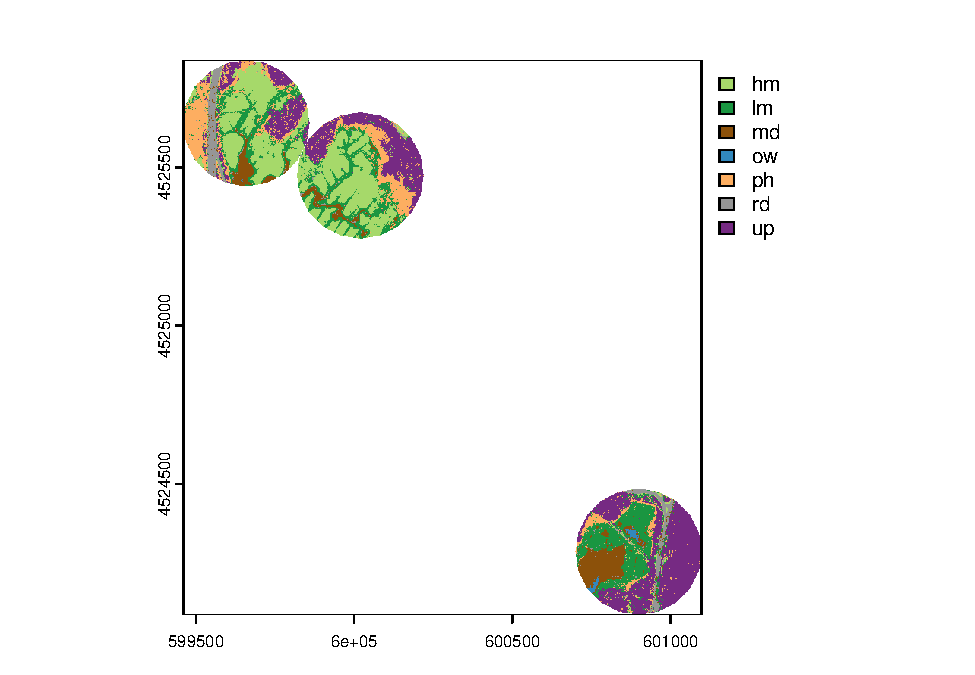
\includegraphics{veg_model_new_class_files/figure-latex/unnamed-chunk-8-1.pdf}

\begin{Shaded}
\begin{Highlighting}[]
\CommentTok{\# save the output tif}
\CommentTok{\# writeRaster(classified, "\textasciitilde{}/Desktop/marshbirdsoutput/round\_6/classified\_output.tif", overwrite = TRUE)}

\NormalTok{model }\OtherTok{\textless{}{-}}\NormalTok{ rf\_model}\SpecialCharTok{$}\NormalTok{importance}
\FunctionTok{print}\NormalTok{(model)}
\end{Highlighting}
\end{Shaded}

\begin{verbatim}
##       MeanDecreaseGini
## naip1         1287.991
## naip2         1177.615
## naip3         1668.540
## naip4         1862.514
## ndvi          1680.766
## ndwi          1915.391
\end{verbatim}

\section{feature class importance and
visualizations}\label{feature-class-importance-and-visualizations-1}

\begin{Shaded}
\begin{Highlighting}[]
\FunctionTok{ggplot}\NormalTok{(training\_data, }\FunctionTok{aes}\NormalTok{(}\AttributeTok{x =}\NormalTok{ naip4, }\AttributeTok{y =}\NormalTok{ ndvi, }\AttributeTok{color =}\NormalTok{ class)) }\SpecialCharTok{+}
  \FunctionTok{geom\_point}\NormalTok{(}\AttributeTok{alpha =} \FloatTok{0.3}\NormalTok{) }\SpecialCharTok{+}
  \FunctionTok{theme\_minimal}\NormalTok{()}
\end{Highlighting}
\end{Shaded}

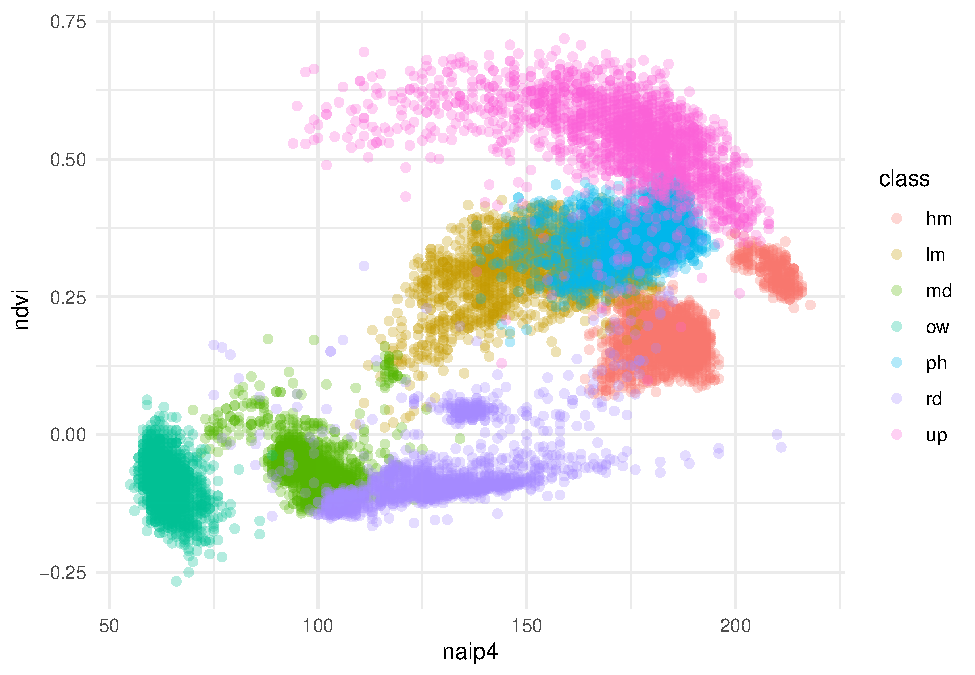
\includegraphics{veg_model_new_class_files/figure-latex/unnamed-chunk-9-1.pdf}

\begin{Shaded}
\begin{Highlighting}[]
\FunctionTok{ggplot}\NormalTok{(training\_data, }\FunctionTok{aes}\NormalTok{(}\AttributeTok{x =}\NormalTok{ naip4, }\AttributeTok{fill =}\NormalTok{ class)) }\SpecialCharTok{+}
  \FunctionTok{geom\_density}\NormalTok{(}\AttributeTok{alpha =} \FloatTok{0.4}\NormalTok{, }\AttributeTok{color =} \ConstantTok{NA}\NormalTok{) }\SpecialCharTok{+}
  \FunctionTok{theme\_minimal}\NormalTok{()}
\end{Highlighting}
\end{Shaded}

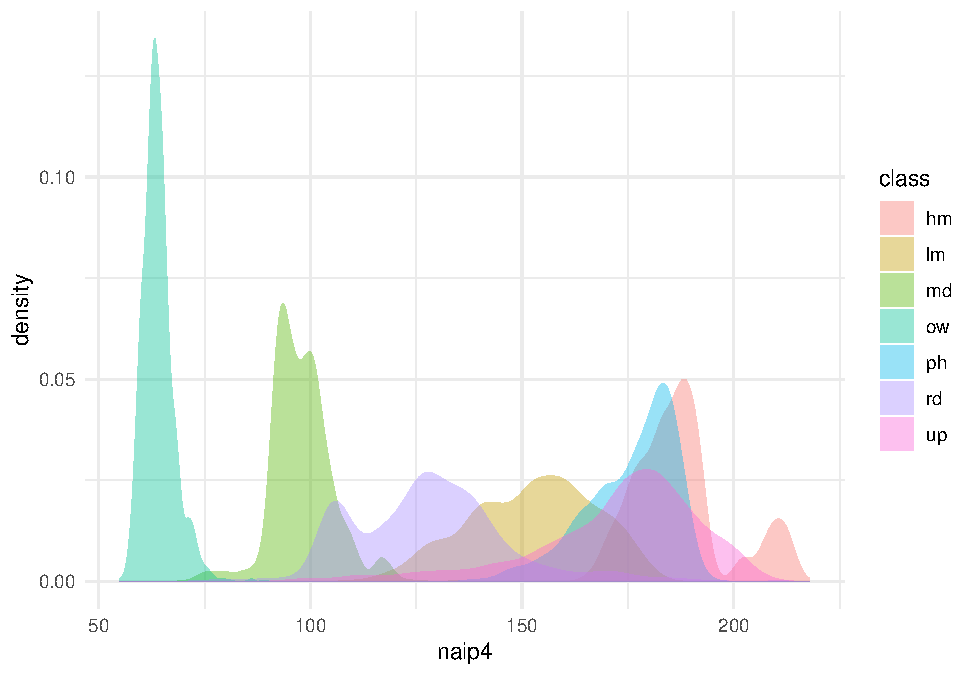
\includegraphics{veg_model_new_class_files/figure-latex/unnamed-chunk-9-2.pdf}

\begin{Shaded}
\begin{Highlighting}[]
\NormalTok{imp }\OtherTok{\textless{}{-}} \FunctionTok{as.data.frame}\NormalTok{(rf\_model}\SpecialCharTok{$}\NormalTok{importance)}
\NormalTok{imp}\SpecialCharTok{$}\NormalTok{feature }\OtherTok{\textless{}{-}} \FunctionTok{rownames}\NormalTok{(imp)}

\FunctionTok{ggplot}\NormalTok{(imp, }\FunctionTok{aes}\NormalTok{(}\AttributeTok{x =} \FunctionTok{reorder}\NormalTok{(feature, MeanDecreaseGini), }\AttributeTok{y =}\NormalTok{ MeanDecreaseGini)) }\SpecialCharTok{+}
  \FunctionTok{geom\_col}\NormalTok{(}\AttributeTok{fill =} \StringTok{"steelblue"}\NormalTok{) }\SpecialCharTok{+}
  \FunctionTok{coord\_flip}\NormalTok{() }\SpecialCharTok{+}
  \FunctionTok{labs}\NormalTok{(}\AttributeTok{title =} \StringTok{"Random Forest Variable Importance"}\NormalTok{,}
       \AttributeTok{x =} \StringTok{"Feature"}\NormalTok{, }\AttributeTok{y =} \StringTok{"Mean Decrease Gini"}\NormalTok{) }\SpecialCharTok{+}
  \FunctionTok{theme\_minimal}\NormalTok{()}
\end{Highlighting}
\end{Shaded}

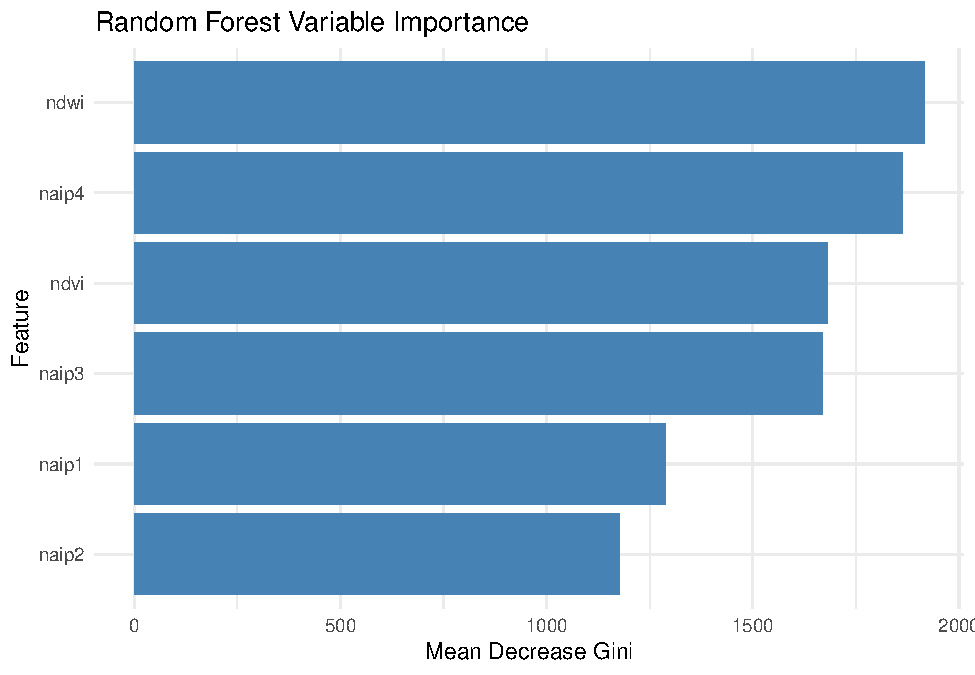
\includegraphics{veg_model_new_class_files/figure-latex/unnamed-chunk-9-3.pdf}

\section{3. Third Iteration: NAIP +
NDVI}\label{third-iteration-naip-ndvi}

\begin{Shaded}
\begin{Highlighting}[]
\CommentTok{\# stack em up}
\NormalTok{r\_stack }\OtherTok{\textless{}{-}} \FunctionTok{c}\NormalTok{(naip, ndvi)}

\CommentTok{\# extract raster values for training polygons}
\NormalTok{extracted }\OtherTok{\textless{}{-}}\NormalTok{ terra}\SpecialCharTok{::}\FunctionTok{extract}\NormalTok{(r\_stack, training\_polygons, }\AttributeTok{df =} \ConstantTok{TRUE}\NormalTok{)}

\CommentTok{\# turn class into a factor}
\NormalTok{training\_polygons}\SpecialCharTok{$}\NormalTok{class }\OtherTok{\textless{}{-}} \FunctionTok{as.factor}\NormalTok{(training\_polygons}\SpecialCharTok{$}\NormalTok{class)}

\CommentTok{\# Convert training\_polygons to dataframe to get the class labels}
\NormalTok{poly\_df }\OtherTok{\textless{}{-}} \FunctionTok{as.data.frame}\NormalTok{(training\_polygons)}
\NormalTok{poly\_df}\SpecialCharTok{$}\NormalTok{ID }\OtherTok{\textless{}{-}} \DecValTok{1}\SpecialCharTok{:}\FunctionTok{nrow}\NormalTok{(poly\_df)  }\CommentTok{\# Add ID column to match extract output}

\CommentTok{\# Join the class labels}
\NormalTok{extracted }\OtherTok{\textless{}{-}}\NormalTok{ extracted }\SpecialCharTok{\%\textgreater{}\%}
  \FunctionTok{left\_join}\NormalTok{(poly\_df[, }\FunctionTok{c}\NormalTok{(}\StringTok{"ID"}\NormalTok{, }\StringTok{"class"}\NormalTok{)], }\AttributeTok{by =} \StringTok{"ID"}\NormalTok{)}

\CommentTok{\# clean data by removing rows with na values and remove ID column}
\NormalTok{extracted\_clean }\OtherTok{\textless{}{-}} \FunctionTok{na.omit}\NormalTok{(extracted[, }\SpecialCharTok{{-}}\DecValTok{1}\NormalTok{])  }\CommentTok{\# remove ID and NAs}

\CommentTok{\# sample 2000 per class}
\NormalTok{training\_data }\OtherTok{\textless{}{-}}\NormalTok{ extracted\_clean }\SpecialCharTok{\%\textgreater{}\%}
  \FunctionTok{group\_by}\NormalTok{(class) }\SpecialCharTok{\%\textgreater{}\%}
  \FunctionTok{sample\_n}\NormalTok{(}\FunctionTok{min}\NormalTok{(}\DecValTok{2000}\NormalTok{, }\FunctionTok{n}\NormalTok{())) }\SpecialCharTok{\%\textgreater{}\%}  \CommentTok{\# Use min() to handle small classes}
  \FunctionTok{ungroup}\NormalTok{()}

\CommentTok{\# turn class column into factor}
\NormalTok{training\_data}\SpecialCharTok{$}\NormalTok{class }\OtherTok{\textless{}{-}} \FunctionTok{factor}\NormalTok{(training\_data}\SpecialCharTok{$}\NormalTok{class)}
\end{Highlighting}
\end{Shaded}

\begin{Shaded}
\begin{Highlighting}[]
\CommentTok{\# split training and test data}
\FunctionTok{set.seed}\NormalTok{(}\DecValTok{342}\NormalTok{)}
\NormalTok{idx }\OtherTok{\textless{}{-}} \FunctionTok{sample}\NormalTok{(}\FunctionTok{seq\_len}\NormalTok{(}\FunctionTok{nrow}\NormalTok{(training\_data)), }\AttributeTok{size =} \FloatTok{0.8} \SpecialCharTok{*} \FunctionTok{nrow}\NormalTok{(training\_data))}
\NormalTok{train\_set }\OtherTok{\textless{}{-}}\NormalTok{ training\_data[idx, ]}
\NormalTok{test\_set  }\OtherTok{\textless{}{-}}\NormalTok{ training\_data[}\SpecialCharTok{{-}}\NormalTok{idx, ]}

\CommentTok{\# train random forest model}
\NormalTok{rf\_model }\OtherTok{\textless{}{-}} \FunctionTok{randomForest}\NormalTok{(class }\SpecialCharTok{\textasciitilde{}}\NormalTok{ ., }
                         \AttributeTok{data =}\NormalTok{ train\_set, }
                         \AttributeTok{ntree =} \DecValTok{500}\NormalTok{)}

\CommentTok{\# validation metrics}
\NormalTok{preds }\OtherTok{\textless{}{-}} \FunctionTok{predict}\NormalTok{(rf\_model, }\AttributeTok{newdata =}\NormalTok{ test\_set)}
\NormalTok{accuracy }\OtherTok{\textless{}{-}} \FunctionTok{mean}\NormalTok{(preds }\SpecialCharTok{==}\NormalTok{ test\_set}\SpecialCharTok{$}\NormalTok{class)}
\FunctionTok{cat}\NormalTok{(}\StringTok{"Accuracy:"}\NormalTok{, }\FunctionTok{round}\NormalTok{(accuracy, }\DecValTok{4}\NormalTok{), }\StringTok{"}\SpecialCharTok{\textbackslash{}n}\StringTok{"}\NormalTok{)}
\end{Highlighting}
\end{Shaded}

\begin{verbatim}
## Accuracy: 0.9686
\end{verbatim}

\begin{Shaded}
\begin{Highlighting}[]
\FunctionTok{print}\NormalTok{(rf\_model)}
\end{Highlighting}
\end{Shaded}

\begin{verbatim}
## 
## Call:
##  randomForest(formula = class ~ ., data = train_set, ntree = 500) 
##                Type of random forest: classification
##                      Number of trees: 500
## No. of variables tried at each split: 2
## 
##         OOB estimate of  error rate: 2.97%
## Confusion matrix:
##      hm   lm   md   ow   ph   rd   up class.error
## hm 1592   11    0    0    0    4    0 0.009334163
## lm   20 1534    3    0   39    0    1 0.039448967
## md    0    1 1551    0    0   49    0 0.031230481
## ow    0    0    1 1587    0    1    0 0.001258653
## ph    0   58    0    0 1535    2   17 0.047766749
## rd    7    4   51    0   13 1530    0 0.046728972
## up    4   17    0    0   28    2 1538 0.032095658
\end{verbatim}

\begin{Shaded}
\begin{Highlighting}[]
\CommentTok{\# confusion matrix}
\FunctionTok{confusionMatrix}\NormalTok{(preds, test\_set}\SpecialCharTok{$}\NormalTok{class)}
\end{Highlighting}
\end{Shaded}

\begin{verbatim}
## Confusion Matrix and Statistics
## 
##           Reference
## Prediction  hm  lm  md  ow  ph  rd  up
##         hm 388   2   0   0   0   3   2
##         lm   4 391   0   0  17   0   5
##         md   0   2 383   1   0  16   0
##         ow   0   0   1 410   0   0   0
##         ph   0   7   0   0 369   2   7
##         rd   1   0  15   0   1 374   0
##         up   0   1   0   0   1   0 397
## 
## Overall Statistics
##                                           
##                Accuracy : 0.9686          
##                  95% CI : (0.9614, 0.9747)
##     No Information Rate : 0.1468          
##     P-Value [Acc > NIR] : < 2.2e-16       
##                                           
##                   Kappa : 0.9633          
##                                           
##  Mcnemar's Test P-Value : NA              
## 
## Statistics by Class:
## 
##                      Class: hm Class: lm Class: md Class: ow Class: ph
## Sensitivity             0.9873    0.9702    0.9599    0.9976    0.9510
## Specificity             0.9971    0.9892    0.9921    0.9996    0.9934
## Pos Pred Value          0.9823    0.9376    0.9527    0.9976    0.9584
## Neg Pred Value          0.9979    0.9950    0.9933    0.9996    0.9921
## Prevalence              0.1404    0.1439    0.1425    0.1468    0.1386
## Detection Rate          0.1386    0.1396    0.1368    0.1464    0.1318
## Detection Prevalence    0.1411    0.1489    0.1436    0.1468    0.1375
## Balanced Accuracy       0.9922    0.9797    0.9760    0.9986    0.9722
##                      Class: rd Class: up
## Sensitivity             0.9468    0.9659
## Specificity             0.9929    0.9992
## Pos Pred Value          0.9565    0.9950
## Neg Pred Value          0.9913    0.9942
## Prevalence              0.1411    0.1468
## Detection Rate          0.1336    0.1418
## Detection Prevalence    0.1396    0.1425
## Balanced Accuracy       0.9699    0.9825
\end{verbatim}

\section{classifying the plots}\label{classifying-the-plots-2}

\begin{Shaded}
\begin{Highlighting}[]
\CommentTok{\# load the new, unlabeled raster}
\NormalTok{prediction\_raster }\OtherTok{\textless{}{-}} \FunctionTok{rast}\NormalTok{(}\StringTok{"\textasciitilde{}/Desktop/marshbirdsoutput/round\_6/prediction\_raster\_round\_6.tif"}\NormalTok{)}

\CommentTok{\# calculate NDVI for prediction raster}
\NormalTok{ndvi\_pred }\OtherTok{\textless{}{-}}\NormalTok{ (prediction\_raster[[}\DecValTok{4}\NormalTok{]] }\SpecialCharTok{{-}}\NormalTok{ prediction\_raster[[}\DecValTok{1}\NormalTok{]]) }\SpecialCharTok{/} 
\NormalTok{  (prediction\_raster[[}\DecValTok{4}\NormalTok{]] }\SpecialCharTok{+}\NormalTok{ prediction\_raster[[}\DecValTok{1}\NormalTok{]])}
\FunctionTok{names}\NormalTok{(ndvi\_pred) }\OtherTok{\textless{}{-}} \StringTok{"ndvi"}

\CommentTok{\# calculation NDWI}
\NormalTok{ndwi\_pred }\OtherTok{\textless{}{-}}\NormalTok{ (prediction\_raster[[}\DecValTok{4}\NormalTok{]] }\SpecialCharTok{{-}}\NormalTok{ prediction\_raster[[}\DecValTok{2}\NormalTok{]]) }\SpecialCharTok{/} 
\NormalTok{  (prediction\_raster[[}\DecValTok{4}\NormalTok{]] }\SpecialCharTok{+}\NormalTok{ prediction\_raster[[}\DecValTok{2}\NormalTok{]])}
\FunctionTok{names}\NormalTok{(ndwi\_pred) }\OtherTok{\textless{}{-}} \StringTok{"ndwi"}

\CommentTok{\# Calculate brightness}
\NormalTok{brightness\_pred }\OtherTok{\textless{}{-}}\NormalTok{ (prediction\_raster[[}\DecValTok{1}\NormalTok{]] }\SpecialCharTok{+}\NormalTok{ prediction\_raster[[}\DecValTok{2}\NormalTok{]] }\SpecialCharTok{+} 
\NormalTok{                      prediction\_raster[[}\DecValTok{3}\NormalTok{]] }\SpecialCharTok{+}\NormalTok{ prediction\_raster[[}\DecValTok{4}\NormalTok{]]) }\SpecialCharTok{/} \DecValTok{4}
\FunctionTok{names}\NormalTok{(brightness\_pred) }\OtherTok{\textless{}{-}} \StringTok{"brightness"}

\CommentTok{\# Apply the pca}
\NormalTok{all\_for\_pca\_pred }\OtherTok{\textless{}{-}} \FunctionTok{c}\NormalTok{(prediction\_raster, ndvi\_pred)}
\FunctionTok{names}\NormalTok{(all\_for\_pca\_pred) }\OtherTok{\textless{}{-}} \FunctionTok{names}\NormalTok{(all\_for\_pca)  }\CommentTok{\# ensure exact match}
\NormalTok{pca\_pred }\OtherTok{\textless{}{-}} \FunctionTok{predict}\NormalTok{(all\_for\_pca\_pred, pca\_pixels, }\AttributeTok{index =} \DecValTok{1}\SpecialCharTok{:}\DecValTok{5}\NormalTok{)}
\end{Highlighting}
\end{Shaded}

\begin{verbatim}
## |---------|---------|---------|---------|=========================================                                          
\end{verbatim}

\begin{Shaded}
\begin{Highlighting}[]
\FunctionTok{names}\NormalTok{(pca\_pred) }\OtherTok{\textless{}{-}} \FunctionTok{paste0}\NormalTok{(}\StringTok{"PCA"}\NormalTok{, }\DecValTok{1}\SpecialCharTok{:}\DecValTok{5}\NormalTok{)}

\CommentTok{\# stack it}
\NormalTok{prediction\_stack }\OtherTok{\textless{}{-}} \FunctionTok{c}\NormalTok{(prediction\_raster, ndvi\_pred)}

\CommentTok{\# rename to match training names}
\FunctionTok{names}\NormalTok{(prediction\_stack) }\OtherTok{\textless{}{-}} \FunctionTok{names}\NormalTok{(r\_stack)}

\CommentTok{\# apply the model to predict classes}
\NormalTok{classified }\OtherTok{\textless{}{-}} \FunctionTok{predict}\NormalTok{(prediction\_stack, rf\_model, }\AttributeTok{na.rm =} \ConstantTok{TRUE}\NormalTok{)}

\CommentTok{\# Define custom colors}
\NormalTok{colors }\OtherTok{\textless{}{-}} \FunctionTok{c}\NormalTok{(}
  \StringTok{"\#a6d96a"}\NormalTok{,  }\CommentTok{\# hm  }
  \StringTok{"\#1a9641"}\NormalTok{,  }\CommentTok{\# lm  }
  \StringTok{"\#8c510a"}\NormalTok{,  }\CommentTok{\# md  }
  \StringTok{"\#3288bd"}\NormalTok{,  }\CommentTok{\# ow  }
  \StringTok{"\#fdae61"}\NormalTok{,  }\CommentTok{\# ph  }
  \StringTok{"\#969696"}\NormalTok{,  }\CommentTok{\# rd  }
  \StringTok{"\#762a83"}   \CommentTok{\# up  }
\NormalTok{)}



\CommentTok{\# Plot with colors}
\FunctionTok{plot}\NormalTok{(classified, }\AttributeTok{col =}\NormalTok{ colors)}
\end{Highlighting}
\end{Shaded}

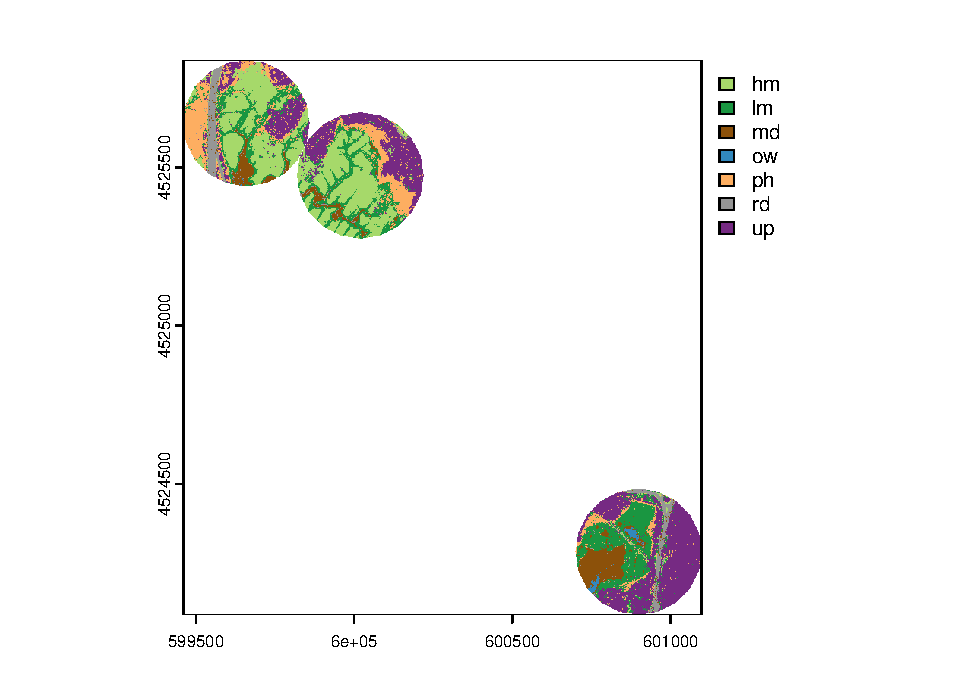
\includegraphics{veg_model_new_class_files/figure-latex/unnamed-chunk-12-1.pdf}

\begin{Shaded}
\begin{Highlighting}[]
\CommentTok{\# save the output tif}
\FunctionTok{writeRaster}\NormalTok{(classified, }\StringTok{"\textasciitilde{}/Desktop/marshbirdsoutput/round\_6/classified\_output.tif"}\NormalTok{, }\AttributeTok{overwrite =} \ConstantTok{TRUE}\NormalTok{)}

\NormalTok{rf\_model}\SpecialCharTok{$}\NormalTok{importance}
\end{Highlighting}
\end{Shaded}

\begin{verbatim}
##       MeanDecreaseGini
## naip1         1469.464
## naip2         1358.500
## naip3         1927.166
## naip4         2286.801
## ndvi          2549.012
\end{verbatim}

\section{feature class importance and
visualizations}\label{feature-class-importance-and-visualizations-2}

\begin{Shaded}
\begin{Highlighting}[]
\FunctionTok{ggplot}\NormalTok{(training\_data, }\FunctionTok{aes}\NormalTok{(}\AttributeTok{x =}\NormalTok{ naip4, }\AttributeTok{y =}\NormalTok{ ndvi, }\AttributeTok{color =}\NormalTok{ class)) }\SpecialCharTok{+}
  \FunctionTok{geom\_point}\NormalTok{(}\AttributeTok{alpha =} \FloatTok{0.3}\NormalTok{) }\SpecialCharTok{+}
  \FunctionTok{theme\_minimal}\NormalTok{()}
\end{Highlighting}
\end{Shaded}

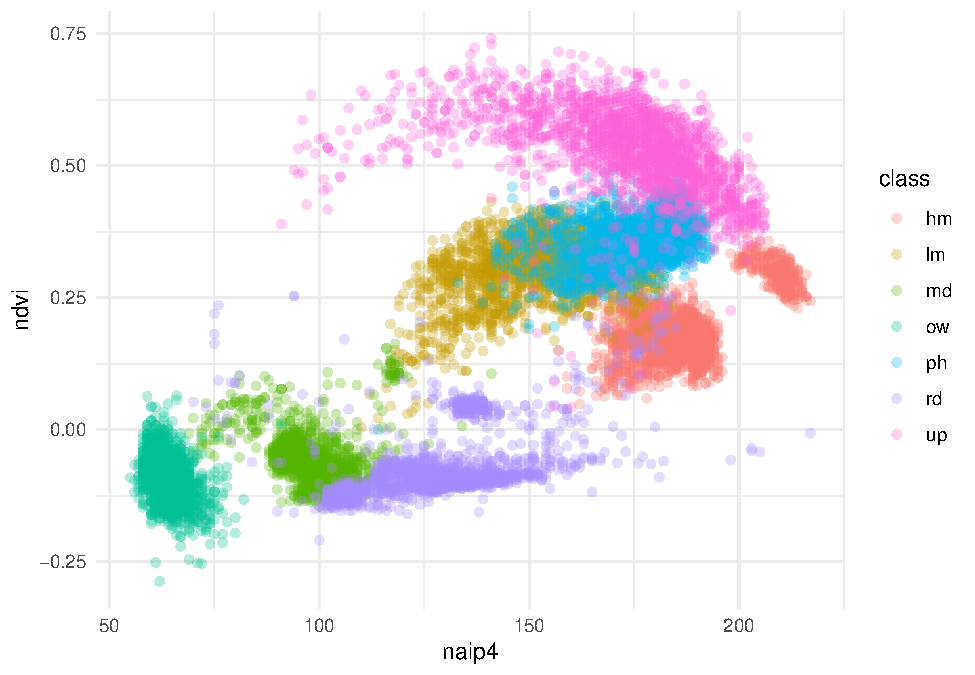
\includegraphics{veg_model_new_class_files/figure-latex/unnamed-chunk-13-1.pdf}

\begin{Shaded}
\begin{Highlighting}[]
\FunctionTok{ggplot}\NormalTok{(training\_data, }\FunctionTok{aes}\NormalTok{(}\AttributeTok{x =}\NormalTok{ naip4, }\AttributeTok{fill =}\NormalTok{ class)) }\SpecialCharTok{+}
  \FunctionTok{geom\_density}\NormalTok{(}\AttributeTok{alpha =} \FloatTok{0.4}\NormalTok{, }\AttributeTok{color =} \ConstantTok{NA}\NormalTok{) }\SpecialCharTok{+}
  \FunctionTok{theme\_minimal}\NormalTok{()}
\end{Highlighting}
\end{Shaded}

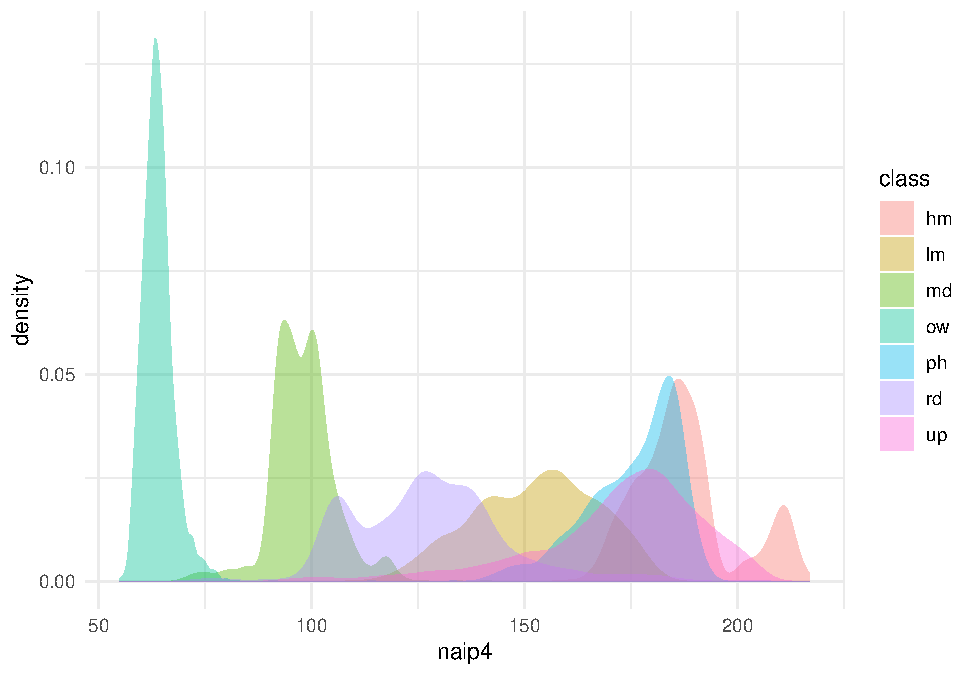
\includegraphics{veg_model_new_class_files/figure-latex/unnamed-chunk-13-2.pdf}

\begin{Shaded}
\begin{Highlighting}[]
\NormalTok{imp }\OtherTok{\textless{}{-}} \FunctionTok{as.data.frame}\NormalTok{(rf\_model}\SpecialCharTok{$}\NormalTok{importance)}
\NormalTok{imp}\SpecialCharTok{$}\NormalTok{feature }\OtherTok{\textless{}{-}} \FunctionTok{rownames}\NormalTok{(imp)}

\FunctionTok{ggplot}\NormalTok{(imp, }\FunctionTok{aes}\NormalTok{(}\AttributeTok{x =} \FunctionTok{reorder}\NormalTok{(feature, MeanDecreaseGini), }\AttributeTok{y =}\NormalTok{ MeanDecreaseGini)) }\SpecialCharTok{+}
  \FunctionTok{geom\_col}\NormalTok{(}\AttributeTok{fill =} \StringTok{"steelblue"}\NormalTok{) }\SpecialCharTok{+}
  \FunctionTok{coord\_flip}\NormalTok{() }\SpecialCharTok{+}
  \FunctionTok{labs}\NormalTok{(}\AttributeTok{title =} \StringTok{"Random Forest Variable Importance"}\NormalTok{,}
       \AttributeTok{x =} \StringTok{"Feature"}\NormalTok{, }\AttributeTok{y =} \StringTok{"Mean Decrease Gini"}\NormalTok{) }\SpecialCharTok{+}
  \FunctionTok{theme\_minimal}\NormalTok{()}
\end{Highlighting}
\end{Shaded}

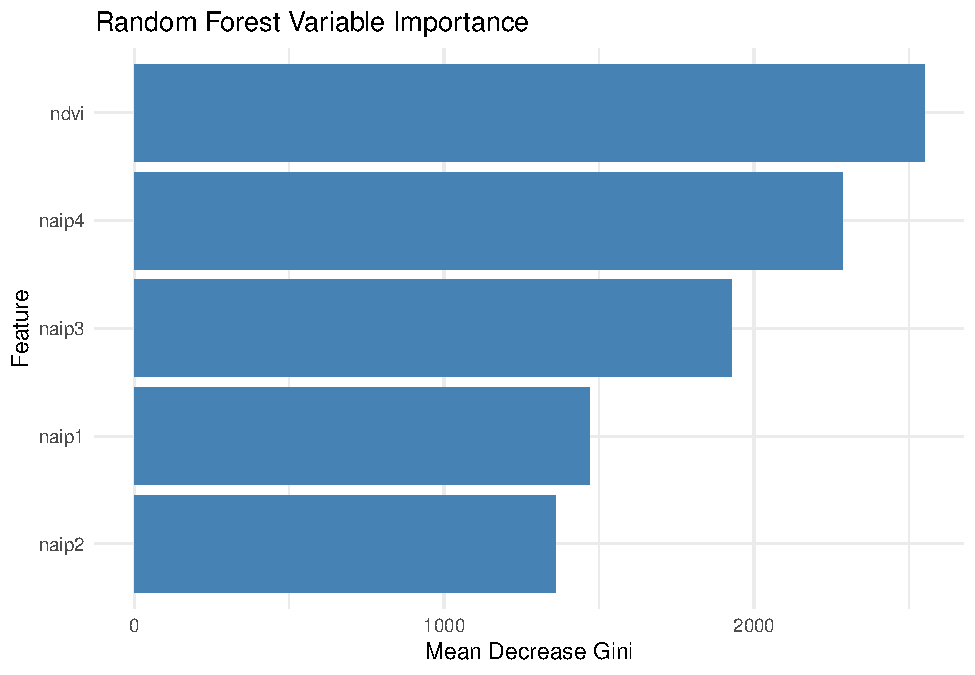
\includegraphics{veg_model_new_class_files/figure-latex/unnamed-chunk-13-3.pdf}

\section{4. Fourth Iteration: PCA}\label{fourth-iteration-pca}

\begin{Shaded}
\begin{Highlighting}[]
\CommentTok{\# stack em up}
\NormalTok{r\_stack }\OtherTok{\textless{}{-}} \FunctionTok{c}\NormalTok{(pca)}

\CommentTok{\# extract raster values for training polygons}
\NormalTok{extracted }\OtherTok{\textless{}{-}}\NormalTok{ terra}\SpecialCharTok{::}\FunctionTok{extract}\NormalTok{(r\_stack, training\_polygons, }\AttributeTok{df =} \ConstantTok{TRUE}\NormalTok{)}

\CommentTok{\# turn class into a factor}
\NormalTok{training\_polygons}\SpecialCharTok{$}\NormalTok{class }\OtherTok{\textless{}{-}} \FunctionTok{as.factor}\NormalTok{(training\_polygons}\SpecialCharTok{$}\NormalTok{class)}

\CommentTok{\# Convert training\_polygons to dataframe to get the class labels}
\NormalTok{poly\_df }\OtherTok{\textless{}{-}} \FunctionTok{as.data.frame}\NormalTok{(training\_polygons)}
\NormalTok{poly\_df}\SpecialCharTok{$}\NormalTok{ID }\OtherTok{\textless{}{-}} \DecValTok{1}\SpecialCharTok{:}\FunctionTok{nrow}\NormalTok{(poly\_df)  }\CommentTok{\# Add ID column to match extract output}

\CommentTok{\# Join the class labels}
\NormalTok{extracted }\OtherTok{\textless{}{-}}\NormalTok{ extracted }\SpecialCharTok{\%\textgreater{}\%}
  \FunctionTok{left\_join}\NormalTok{(poly\_df[, }\FunctionTok{c}\NormalTok{(}\StringTok{"ID"}\NormalTok{, }\StringTok{"class"}\NormalTok{)], }\AttributeTok{by =} \StringTok{"ID"}\NormalTok{)}

\CommentTok{\# clean data by removing rows with na values and remove ID column}
\NormalTok{extracted\_clean }\OtherTok{\textless{}{-}} \FunctionTok{na.omit}\NormalTok{(extracted[, }\SpecialCharTok{{-}}\DecValTok{1}\NormalTok{])  }\CommentTok{\# remove ID and NAs}

\CommentTok{\# sample 2000 per class}
\NormalTok{training\_data }\OtherTok{\textless{}{-}}\NormalTok{ extracted\_clean }\SpecialCharTok{\%\textgreater{}\%}
  \FunctionTok{group\_by}\NormalTok{(class) }\SpecialCharTok{\%\textgreater{}\%}
  \FunctionTok{sample\_n}\NormalTok{(}\FunctionTok{min}\NormalTok{(}\DecValTok{2000}\NormalTok{, }\FunctionTok{n}\NormalTok{())) }\SpecialCharTok{\%\textgreater{}\%}  \CommentTok{\# Use min() to handle small classes}
  \FunctionTok{ungroup}\NormalTok{()}

\CommentTok{\# turn class column into factor}
\NormalTok{training\_data}\SpecialCharTok{$}\NormalTok{class }\OtherTok{\textless{}{-}} \FunctionTok{factor}\NormalTok{(training\_data}\SpecialCharTok{$}\NormalTok{class)}
\end{Highlighting}
\end{Shaded}

\section{check the sampling balance in the
classes}\label{check-the-sampling-balance-in-the-classes}

\section{print(``Class distribution in training
data:'')}\label{printclass-distribution-in-training-data}

\section{print(table(training\_data\$class))}\label{printtabletraining_dataclass}

\begin{Shaded}
\begin{Highlighting}[]
\CommentTok{\# split training and test data}
\FunctionTok{set.seed}\NormalTok{(}\DecValTok{342}\NormalTok{)}
\NormalTok{idx }\OtherTok{\textless{}{-}} \FunctionTok{sample}\NormalTok{(}\FunctionTok{seq\_len}\NormalTok{(}\FunctionTok{nrow}\NormalTok{(training\_data)), }\AttributeTok{size =} \FloatTok{0.8} \SpecialCharTok{*} \FunctionTok{nrow}\NormalTok{(training\_data))}
\NormalTok{train\_set }\OtherTok{\textless{}{-}}\NormalTok{ training\_data[idx, ]}
\NormalTok{test\_set  }\OtherTok{\textless{}{-}}\NormalTok{ training\_data[}\SpecialCharTok{{-}}\NormalTok{idx, ]}

\CommentTok{\# train random forest model}
\NormalTok{rf\_model }\OtherTok{\textless{}{-}} \FunctionTok{randomForest}\NormalTok{(class }\SpecialCharTok{\textasciitilde{}}\NormalTok{ ., }
                         \AttributeTok{data =}\NormalTok{ train\_set, }
                         \AttributeTok{ntree =} \DecValTok{500}\NormalTok{)}

\CommentTok{\# validation metrics}
\NormalTok{preds }\OtherTok{\textless{}{-}} \FunctionTok{predict}\NormalTok{(rf\_model, }\AttributeTok{newdata =}\NormalTok{ test\_set)}
\NormalTok{accuracy }\OtherTok{\textless{}{-}} \FunctionTok{mean}\NormalTok{(preds }\SpecialCharTok{==}\NormalTok{ test\_set}\SpecialCharTok{$}\NormalTok{class)}
\FunctionTok{cat}\NormalTok{(}\StringTok{"Accuracy:"}\NormalTok{, }\FunctionTok{round}\NormalTok{(accuracy, }\DecValTok{4}\NormalTok{), }\StringTok{"}\SpecialCharTok{\textbackslash{}n}\StringTok{"}\NormalTok{)}
\end{Highlighting}
\end{Shaded}

\begin{verbatim}
## Accuracy: 0.9779
\end{verbatim}

\begin{Shaded}
\begin{Highlighting}[]
\FunctionTok{print}\NormalTok{(rf\_model)}
\end{Highlighting}
\end{Shaded}

\begin{verbatim}
## 
## Call:
##  randomForest(formula = class ~ ., data = train_set, ntree = 500) 
##                Type of random forest: classification
##                      Number of trees: 500
## No. of variables tried at each split: 2
## 
##         OOB estimate of  error rate: 2.67%
## Confusion matrix:
##      hm   lm   md   ow   ph   rd   up class.error
## hm 1592   12    0    0    0    2    1 0.009334163
## lm   18 1539    5    0   32    0    3 0.036318096
## md    0    2 1554    2    0   43    0 0.029356652
## ow    0    0    5 1583    0    1    0 0.003775960
## ph    0   44    0    0 1542    1   25 0.043424318
## rd    2    0   40    0   11 1552    0 0.033021807
## up    2   24    0    0   23    1 1539 0.031466331
\end{verbatim}

\begin{Shaded}
\begin{Highlighting}[]
\CommentTok{\# confusion matrix}
\FunctionTok{confusionMatrix}\NormalTok{(preds, test\_set}\SpecialCharTok{$}\NormalTok{class)}
\end{Highlighting}
\end{Shaded}

\begin{verbatim}
## Confusion Matrix and Statistics
## 
##           Reference
## Prediction  hm  lm  md  ow  ph  rd  up
##         hm 393   4   0   0   0   0   0
##         lm   0 390   0   0  13   0   2
##         md   0   0 389   4   0   6   0
##         ow   0   0   1 407   0   0   0
##         ph   0   8   1   0 373   4   8
##         rd   0   0   8   0   0 385   0
##         up   0   1   0   0   2   0 401
## 
## Overall Statistics
##                                          
##                Accuracy : 0.9779         
##                  95% CI : (0.9717, 0.983)
##     No Information Rate : 0.1468         
##     P-Value [Acc > NIR] : < 2.2e-16      
##                                          
##                   Kappa : 0.9742         
##                                          
##  Mcnemar's Test P-Value : NA             
## 
## Statistics by Class:
## 
##                      Class: hm Class: lm Class: md Class: ow Class: ph
## Sensitivity             1.0000    0.9677    0.9749    0.9903    0.9613
## Specificity             0.9983    0.9937    0.9958    0.9996    0.9913
## Pos Pred Value          0.9899    0.9630    0.9749    0.9975    0.9467
## Neg Pred Value          1.0000    0.9946    0.9958    0.9983    0.9938
## Prevalence              0.1404    0.1439    0.1425    0.1468    0.1386
## Detection Rate          0.1404    0.1393    0.1389    0.1454    0.1332
## Detection Prevalence    0.1418    0.1446    0.1425    0.1457    0.1407
## Balanced Accuracy       0.9992    0.9807    0.9854    0.9949    0.9763
##                      Class: rd Class: up
## Sensitivity             0.9747    0.9757
## Specificity             0.9967    0.9987
## Pos Pred Value          0.9796    0.9926
## Neg Pred Value          0.9958    0.9958
## Prevalence              0.1411    0.1468
## Detection Rate          0.1375    0.1432
## Detection Prevalence    0.1404    0.1443
## Balanced Accuracy       0.9857    0.9872
\end{verbatim}

\section{classifying the plots}\label{classifying-the-plots-3}

\begin{Shaded}
\begin{Highlighting}[]
\CommentTok{\# load the new, unlabeled raster}
\NormalTok{prediction\_raster }\OtherTok{\textless{}{-}} \FunctionTok{rast}\NormalTok{(}\StringTok{"\textasciitilde{}/Desktop/marshbirdsoutput/round\_6/prediction\_raster\_round\_6.tif"}\NormalTok{)}

\CommentTok{\# calculate NDVI for prediction raster}
\NormalTok{ndvi\_pred }\OtherTok{\textless{}{-}}\NormalTok{ (prediction\_raster[[}\DecValTok{4}\NormalTok{]] }\SpecialCharTok{{-}}\NormalTok{ prediction\_raster[[}\DecValTok{1}\NormalTok{]]) }\SpecialCharTok{/} 
\NormalTok{  (prediction\_raster[[}\DecValTok{4}\NormalTok{]] }\SpecialCharTok{+}\NormalTok{ prediction\_raster[[}\DecValTok{1}\NormalTok{]])}
\FunctionTok{names}\NormalTok{(ndvi\_pred) }\OtherTok{\textless{}{-}} \StringTok{"ndvi"}

\CommentTok{\# calculation NDWI}
\NormalTok{ndwi\_pred }\OtherTok{\textless{}{-}}\NormalTok{ (prediction\_raster[[}\DecValTok{4}\NormalTok{]] }\SpecialCharTok{{-}}\NormalTok{ prediction\_raster[[}\DecValTok{2}\NormalTok{]]) }\SpecialCharTok{/} 
\NormalTok{  (prediction\_raster[[}\DecValTok{4}\NormalTok{]] }\SpecialCharTok{+}\NormalTok{ prediction\_raster[[}\DecValTok{2}\NormalTok{]])}
\FunctionTok{names}\NormalTok{(ndwi\_pred) }\OtherTok{\textless{}{-}} \StringTok{"ndwi"}

\CommentTok{\# Calculate brightness}
\NormalTok{brightness\_pred }\OtherTok{\textless{}{-}}\NormalTok{ (prediction\_raster[[}\DecValTok{1}\NormalTok{]] }\SpecialCharTok{+}\NormalTok{ prediction\_raster[[}\DecValTok{2}\NormalTok{]] }\SpecialCharTok{+} 
\NormalTok{                      prediction\_raster[[}\DecValTok{3}\NormalTok{]] }\SpecialCharTok{+}\NormalTok{ prediction\_raster[[}\DecValTok{4}\NormalTok{]]) }\SpecialCharTok{/} \DecValTok{4}
\FunctionTok{names}\NormalTok{(brightness\_pred) }\OtherTok{\textless{}{-}} \StringTok{"brightness"}

\CommentTok{\# Apply the pca}
\NormalTok{all\_for\_pca\_pred }\OtherTok{\textless{}{-}} \FunctionTok{c}\NormalTok{(prediction\_raster, ndvi\_pred)}
\FunctionTok{names}\NormalTok{(all\_for\_pca\_pred) }\OtherTok{\textless{}{-}} \FunctionTok{names}\NormalTok{(all\_for\_pca)  }\CommentTok{\# ensure exact match}
\NormalTok{pca\_pred }\OtherTok{\textless{}{-}} \FunctionTok{predict}\NormalTok{(all\_for\_pca\_pred, pca\_pixels, }\AttributeTok{index =} \DecValTok{1}\SpecialCharTok{:}\DecValTok{5}\NormalTok{)}
\end{Highlighting}
\end{Shaded}

\begin{verbatim}
## |---------|---------|---------|---------|=========================================                                          
\end{verbatim}

\begin{Shaded}
\begin{Highlighting}[]
\FunctionTok{names}\NormalTok{(pca\_pred) }\OtherTok{\textless{}{-}} \FunctionTok{paste0}\NormalTok{(}\StringTok{"PCA"}\NormalTok{, }\DecValTok{1}\SpecialCharTok{:}\DecValTok{5}\NormalTok{)}

\CommentTok{\# stack it}
\NormalTok{prediction\_stack }\OtherTok{\textless{}{-}} \FunctionTok{c}\NormalTok{(pca\_pred)}

\CommentTok{\# rename to match training names}
\FunctionTok{names}\NormalTok{(prediction\_stack) }\OtherTok{\textless{}{-}} \FunctionTok{names}\NormalTok{(r\_stack)}

\CommentTok{\# apply the model to predict classes}
\NormalTok{classified }\OtherTok{\textless{}{-}} \FunctionTok{predict}\NormalTok{(prediction\_stack, rf\_model, }\AttributeTok{na.rm =} \ConstantTok{TRUE}\NormalTok{)}

\CommentTok{\# Define custom colors}
\NormalTok{colors }\OtherTok{\textless{}{-}} \FunctionTok{c}\NormalTok{(}
  \StringTok{"\#a6d96a"}\NormalTok{,  }\CommentTok{\# hm  }
  \StringTok{"\#1a9641"}\NormalTok{,  }\CommentTok{\# lm  }
  \StringTok{"\#8c510a"}\NormalTok{,  }\CommentTok{\# md  }
  \StringTok{"\#3288bd"}\NormalTok{,  }\CommentTok{\# ow  }
  \StringTok{"\#fdae61"}\NormalTok{,  }\CommentTok{\# ph  }
  \StringTok{"\#969696"}\NormalTok{,  }\CommentTok{\# rd  }
  \StringTok{"\#762a83"}   \CommentTok{\# up  }
\NormalTok{)}



\CommentTok{\# Plot with colors}
\FunctionTok{plot}\NormalTok{(classified, }\AttributeTok{col =}\NormalTok{ colors)}
\end{Highlighting}
\end{Shaded}

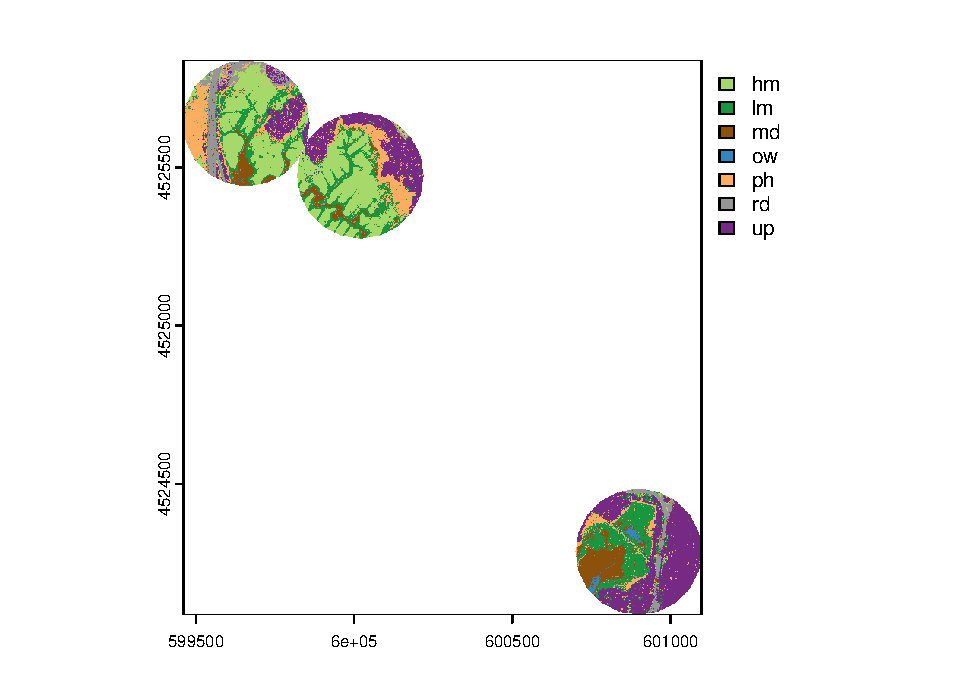
\includegraphics{veg_model_new_class_files/figure-latex/unnamed-chunk-16-1.pdf}

\begin{Shaded}
\begin{Highlighting}[]
\CommentTok{\# save the output tif}
\FunctionTok{writeRaster}\NormalTok{(classified, }\StringTok{"\textasciitilde{}/Desktop/marshbirdsoutput/round\_6/classified\_output.tif"}\NormalTok{, }\AttributeTok{overwrite =} \ConstantTok{TRUE}\NormalTok{)}

\NormalTok{rf\_model}\SpecialCharTok{$}\NormalTok{importance}
\end{Highlighting}
\end{Shaded}

\begin{verbatim}
##      MeanDecreaseGini
## PCA1        3245.3535
## PCA2        2769.8979
## PCA3        1849.6364
## PCA4         808.6667
## PCA5         925.0009
\end{verbatim}

\section{feature class importance and
visualizations}\label{feature-class-importance-and-visualizations-3}

\begin{Shaded}
\begin{Highlighting}[]
\FunctionTok{ggplot}\NormalTok{(training\_data, }\FunctionTok{aes}\NormalTok{(}\AttributeTok{x =}\NormalTok{ PCA3, }\AttributeTok{y =}\NormalTok{ PCA1, }\AttributeTok{color =}\NormalTok{ class)) }\SpecialCharTok{+}
  \FunctionTok{geom\_point}\NormalTok{(}\AttributeTok{alpha =} \FloatTok{0.3}\NormalTok{) }\SpecialCharTok{+}
  \FunctionTok{theme\_minimal}\NormalTok{()}
\end{Highlighting}
\end{Shaded}

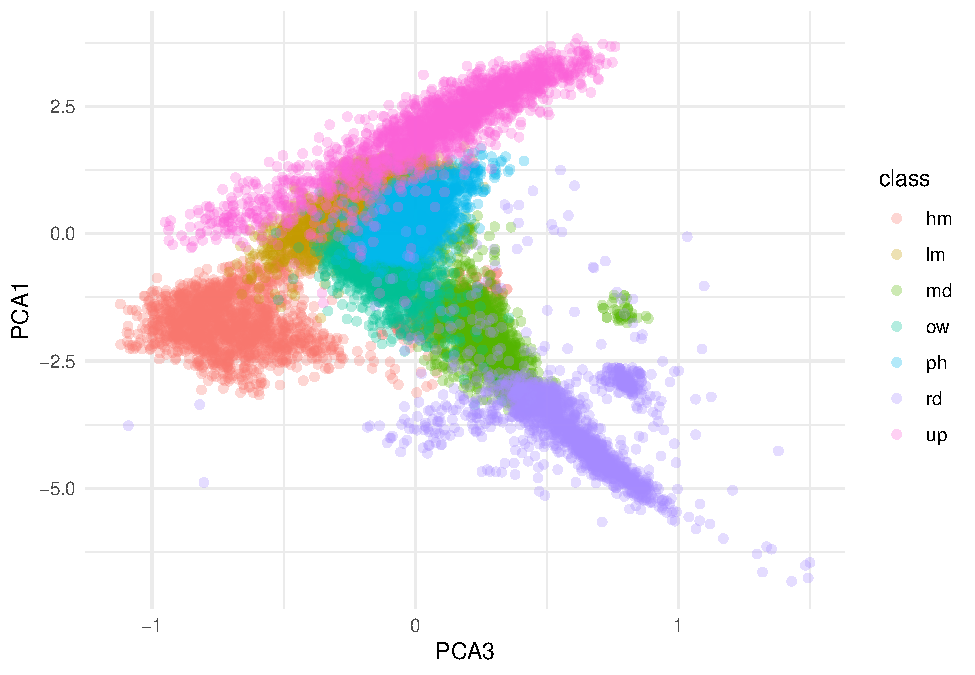
\includegraphics{veg_model_new_class_files/figure-latex/unnamed-chunk-17-1.pdf}

\begin{Shaded}
\begin{Highlighting}[]
\FunctionTok{ggplot}\NormalTok{(training\_data, }\FunctionTok{aes}\NormalTok{(}\AttributeTok{x =}\NormalTok{ PCA1, }\AttributeTok{fill =}\NormalTok{ class)) }\SpecialCharTok{+}
  \FunctionTok{geom\_density}\NormalTok{(}\AttributeTok{alpha =} \FloatTok{0.4}\NormalTok{, }\AttributeTok{color =} \ConstantTok{NA}\NormalTok{) }\SpecialCharTok{+}
  \FunctionTok{theme\_minimal}\NormalTok{()}
\end{Highlighting}
\end{Shaded}

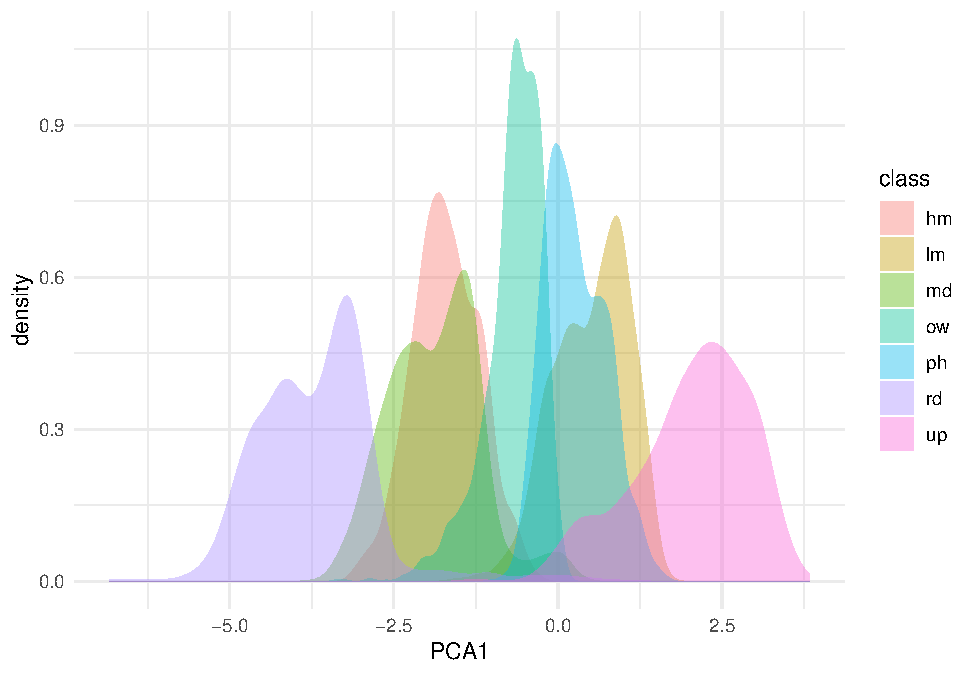
\includegraphics{veg_model_new_class_files/figure-latex/unnamed-chunk-17-2.pdf}

\begin{Shaded}
\begin{Highlighting}[]
\NormalTok{imp }\OtherTok{\textless{}{-}} \FunctionTok{as.data.frame}\NormalTok{(rf\_model}\SpecialCharTok{$}\NormalTok{importance)}
\NormalTok{imp}\SpecialCharTok{$}\NormalTok{feature }\OtherTok{\textless{}{-}} \FunctionTok{rownames}\NormalTok{(imp)}

\FunctionTok{ggplot}\NormalTok{(imp, }\FunctionTok{aes}\NormalTok{(}\AttributeTok{x =} \FunctionTok{reorder}\NormalTok{(feature, MeanDecreaseGini), }\AttributeTok{y =}\NormalTok{ MeanDecreaseGini)) }\SpecialCharTok{+}
  \FunctionTok{geom\_col}\NormalTok{(}\AttributeTok{fill =} \StringTok{"steelblue"}\NormalTok{) }\SpecialCharTok{+}
  \FunctionTok{coord\_flip}\NormalTok{() }\SpecialCharTok{+}
  \FunctionTok{labs}\NormalTok{(}\AttributeTok{title =} \StringTok{"Random Forest Variable Importance"}\NormalTok{,}
       \AttributeTok{x =} \StringTok{"Feature"}\NormalTok{, }\AttributeTok{y =} \StringTok{"Mean Decrease Gini"}\NormalTok{) }\SpecialCharTok{+}
  \FunctionTok{theme\_minimal}\NormalTok{()}
\end{Highlighting}
\end{Shaded}

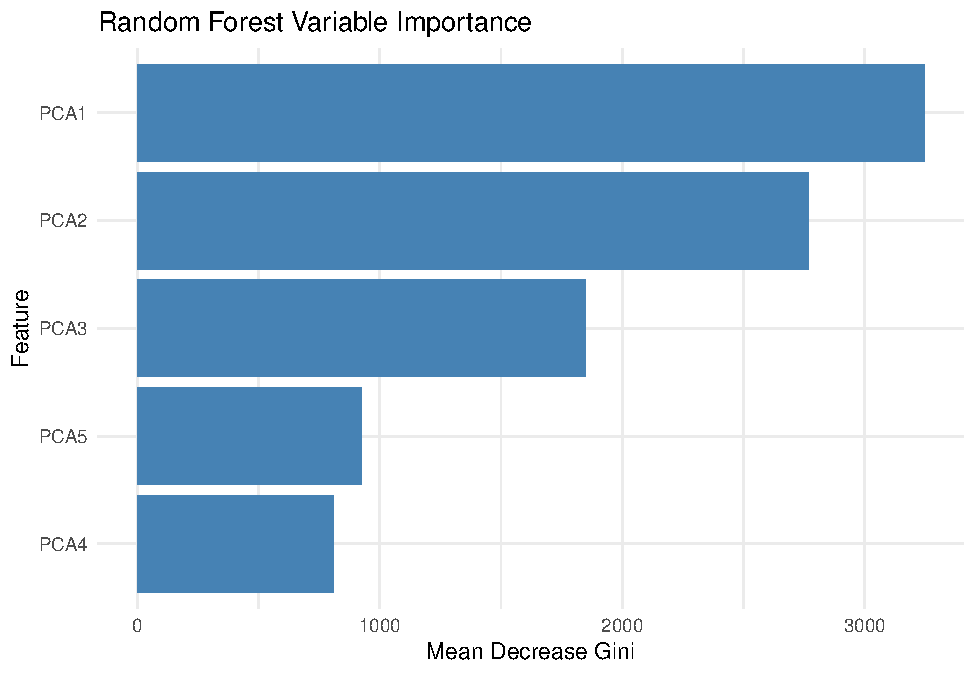
\includegraphics{veg_model_new_class_files/figure-latex/unnamed-chunk-17-3.pdf}

\end{document}
